\documentclass[twoside]{book}

% Packages required by doxygen
\usepackage{calc}
\usepackage{doxygen}
\usepackage{graphicx}
\usepackage[utf8]{inputenc}
\usepackage{makeidx}
\usepackage{multicol}
\usepackage{multirow}
\usepackage{textcomp}
\usepackage[table]{xcolor}

% Font selection
\usepackage[T1]{fontenc}
\usepackage{mathptmx}
\usepackage[scaled=.90]{helvet}
\usepackage{courier}
\usepackage{amssymb}
\usepackage{sectsty}
\renewcommand{\familydefault}{\sfdefault}
\allsectionsfont{%
  \fontseries{bc}\selectfont%
  \color{darkgray}%
}
\renewcommand{\DoxyLabelFont}{%
  \fontseries{bc}\selectfont%
  \color{darkgray}%
}

% Page & text layout
\usepackage{geometry}
\geometry{%
  a4paper,%
  top=2.5cm,%
  bottom=2.5cm,%
  left=2.5cm,%
  right=2.5cm%
}
\tolerance=750
\hfuzz=15pt
\hbadness=750
\setlength{\emergencystretch}{15pt}
\setlength{\parindent}{0cm}
\setlength{\parskip}{0.2cm}
\makeatletter
\renewcommand{\paragraph}{%
  \@startsection{paragraph}{4}{0ex}{-1.0ex}{1.0ex}{%
    \normalfont\normalsize\bfseries\SS@parafont%
  }%
}
\renewcommand{\subparagraph}{%
  \@startsection{subparagraph}{5}{0ex}{-1.0ex}{1.0ex}{%
    \normalfont\normalsize\bfseries\SS@subparafont%
  }%
}
\makeatother

% Headers & footers
\usepackage{fancyhdr}
\pagestyle{fancyplain}
\fancyhead[LE]{\fancyplain{}{\bfseries\thepage}}
\fancyhead[CE]{\fancyplain{}{}}
\fancyhead[RE]{\fancyplain{}{\bfseries\leftmark}}
\fancyhead[LO]{\fancyplain{}{\bfseries\rightmark}}
\fancyhead[CO]{\fancyplain{}{}}
\fancyhead[RO]{\fancyplain{}{\bfseries\thepage}}
\fancyfoot[LE]{\fancyplain{}{}}
\fancyfoot[CE]{\fancyplain{}{}}
\fancyfoot[RE]{\fancyplain{}{\bfseries\scriptsize Generated on Mon May 22 2017 16\-:00\-:07 for My Project by Doxygen }}
\fancyfoot[LO]{\fancyplain{}{\bfseries\scriptsize Generated on Mon May 22 2017 16\-:00\-:07 for My Project by Doxygen }}
\fancyfoot[CO]{\fancyplain{}{}}
\fancyfoot[RO]{\fancyplain{}{}}
\renewcommand{\footrulewidth}{0.4pt}
\renewcommand{\chaptermark}[1]{%
  \markboth{#1}{}%
}
\renewcommand{\sectionmark}[1]{%
  \markright{\thesection\ #1}%
}

% Indices & bibliography
\usepackage{natbib}
\usepackage[titles]{tocloft}
\setcounter{tocdepth}{3}
\setcounter{secnumdepth}{5}
\makeindex

% Hyperlinks (required, but should be loaded last)
\usepackage{ifpdf}
\ifpdf
  \usepackage[pdftex,pagebackref=true]{hyperref}
\else
  \usepackage[ps2pdf,pagebackref=true]{hyperref}
\fi
\hypersetup{%
  colorlinks=true,%
  linkcolor=blue,%
  citecolor=blue,%
  unicode%
}

% Custom commands
\newcommand{\clearemptydoublepage}{%
  \newpage{\pagestyle{empty}\cleardoublepage}%
}


%===== C O N T E N T S =====

\begin{document}

% Titlepage & ToC
\hypersetup{pageanchor=false}
\pagenumbering{roman}
\begin{titlepage}
\vspace*{7cm}
\begin{center}%
{\Large My Project }\\
\vspace*{1cm}
{\large Generated by Doxygen 1.8.6}\\
\vspace*{0.5cm}
{\small Mon May 22 2017 16:00:07}\\
\end{center}
\end{titlepage}
\clearemptydoublepage
\tableofcontents
\clearemptydoublepage
\pagenumbering{arabic}
\hypersetup{pageanchor=true}

%--- Begin generated contents ---
\chapter{Hierarchical Index}
\section{Class Hierarchy}
This inheritance list is sorted roughly, but not completely, alphabetically\-:\begin{DoxyCompactList}
\item \contentsline{section}{Base\-Gfx\-App}{\pageref{classBaseGfxApp}}{}
\begin{DoxyCompactList}
\item \contentsline{section}{Simulation}{\pageref{classSimulation}}{}
\end{DoxyCompactList}
\item \contentsline{section}{Base\-Object}{\pageref{classBaseObject}}{}
\begin{DoxyCompactList}
\item \contentsline{section}{Obstacle}{\pageref{classObstacle}}{}
\item \contentsline{section}{Robot}{\pageref{classRobot}}{}
\item \contentsline{section}{Target}{\pageref{classTarget}}{}
\end{DoxyCompactList}
\item \contentsline{section}{Environment}{\pageref{classEnvironment}}{}
\item Test\-Suite\begin{DoxyCompactList}
\item \contentsline{section}{Environment\-Tests}{\pageref{classEnvironmentTests}}{}
\item \contentsline{section}{Robot\-Tests}{\pageref{classRobotTests}}{}
\end{DoxyCompactList}
\item \contentsline{section}{Walls}{\pageref{classWalls}}{}
\end{DoxyCompactList}

\chapter{Class Index}
\section{Class List}
Here are the classes, structs, unions and interfaces with brief descriptions\-:\begin{DoxyCompactList}
\item\contentsline{section}{\hyperlink{classBaseGfxApp}{Base\-Gfx\-App} }{\pageref{classBaseGfxApp}}{}
\item\contentsline{section}{\hyperlink{classBaseObject}{Base\-Object} }{\pageref{classBaseObject}}{}
\item\contentsline{section}{\hyperlink{classEnvironment}{Environment} }{\pageref{classEnvironment}}{}
\item\contentsline{section}{\hyperlink{classEnvironmentTests}{Environment\-Tests} }{\pageref{classEnvironmentTests}}{}
\item\contentsline{section}{\hyperlink{classObstacle}{Obstacle} }{\pageref{classObstacle}}{}
\item\contentsline{section}{\hyperlink{classRobot}{Robot} }{\pageref{classRobot}}{}
\item\contentsline{section}{\hyperlink{classRobotTests}{Robot\-Tests} }{\pageref{classRobotTests}}{}
\item\contentsline{section}{\hyperlink{classSimulation}{Simulation} }{\pageref{classSimulation}}{}
\item\contentsline{section}{\hyperlink{classTarget}{Target} }{\pageref{classTarget}}{}
\item\contentsline{section}{\hyperlink{classWalls}{Walls} }{\pageref{classWalls}}{}
\end{DoxyCompactList}

\chapter{File Index}
\section{File List}
Here is a list of all documented files with brief descriptions\-:\begin{DoxyCompactList}
\item\contentsline{section}{\hyperlink{BaseGfxApp_8hpp}{Base\-Gfx\-App.\-hpp} \\*The basic application class for C\-Sci-\/3081 project. Uses G\-L\-U\-T and G\-L\-U\-I and wraps them in a nice C++ interface }{\pageref{BaseGfxApp_8hpp}}{}
\item\contentsline{section}{\hyperlink{BaseObject_8hpp}{Base\-Object.\-hpp} \\*The base class which all other physical objects derive from. It contains core data relevant to all objects, such as speed, size, color, object id number, and collision logic }{\pageref{BaseObject_8hpp}}{}
\item\contentsline{section}{\hyperlink{Environment_8hpp}{Environment.\-hpp} \\*The declaration for the enviromnet class. This class explain to update and touch sensor and homing sensor. This class serves as a parent for Physical object Class, The physical object class include collisionstatus, object color, radius, and orientaion }{\pageref{Environment_8hpp}}{}
\item\contentsline{section}{{\bfseries Environment\-Tests.\-hpp} }{\pageref{EnvironmentTests_8hpp}}{}
\item\contentsline{section}{\hyperlink{main_8cpp}{main.\-cpp} \\*Main function }{\pageref{main_8cpp}}{}
\item\contentsline{section}{\hyperlink{Obstacle_8cpp}{Obstacle.\-cpp} \\*Class definition for the \hyperlink{classObstacle}{Obstacle} (child class of \hyperlink{classEnvironment}{Environment}). An obstacle inherits all of its methods from its parent. Improving the code, obstacles have their own unique methods and data. \hyperlink{classEnvironment}{Environment} Class \hyperlink{classEnvironment}{Environment} with static data structure that hold obstacle objects.\-Iteration through the object and moving them based on elasped\-Time }{\pageref{Obstacle_8cpp}}{}
\item\contentsline{section}{{\bfseries Obstacle.\-hpp} }{\pageref{Obstacle_8hpp}}{}
\item\contentsline{section}{\hyperlink{Robot_8cpp}{Robot.\-cpp} \\*A robot inherits much of its methods from its parent. However, it also extends it by adding robot-\/specific methods such as point\-To, which points the robot at a target. Future functionality will have the robot controlled by the user physically pressing keys, which will be distinct from how other agents are manipulated }{\pageref{Robot_8cpp}}{}
\item\contentsline{section}{\hyperlink{Robot_8hpp}{Robot.\-hpp} \\*Class definition for the \hyperlink{classRobot}{Robot} (child class of \hyperlink{classEnvironment}{Environment}). A robot inherits much of its methods from its parent. However, it also extends it by adding robot-\/specific methods such as point\-To, which points the robot at a target. Improving the iteration 2 code, \hyperlink{classRobot}{Robot} adding to sensor about touch and homing. Being able to collide obstacle, \hyperlink{classRobot}{Robot} adding to recognize the target and obstacle }{\pageref{Robot_8hpp}}{}
\item\contentsline{section}{{\bfseries Robot\-Tests.\-hpp} }{\pageref{RobotTests_8hpp}}{}
\item\contentsline{section}{\hyperlink{Simulation_8cpp}{Simulation.\-cpp} \\*Main application class for the robot simulation }{\pageref{Simulation_8cpp}}{}
\item\contentsline{section}{\hyperlink{Simulation_8hpp}{Simulation.\-hpp} \\*Main application class for the robot simulation }{\pageref{Simulation_8hpp}}{}
\item\contentsline{section}{\hyperlink{Target_8cpp}{Target.\-cpp} \\*Objects of this type will be targets that the robot points to. A target inherits all of its methods from its parent. However, in the future targets may have their own unique methods and data }{\pageref{Target_8cpp}}{}
\item\contentsline{section}{\hyperlink{Target_8hpp}{Target.\-hpp} \\*Class definition for the \hyperlink{classTarget}{Target} (child class of \hyperlink{classEnvironment}{Environment}). An Objects of this type will be targets that the robot points to. A target inherits all of its methods from its parent. Improving the code, targets may have their own unique methods and data. \hyperlink{classEnvironment}{Environment} Class \hyperlink{classEnvironment}{Environment} with static data structure that hold target objects.\-Checking Enviroment\-Class update function }{\pageref{Target_8hpp}}{}
\item\contentsline{section}{\hyperlink{Walls_8cpp}{Walls.\-cpp} \\*Class definition for the \hyperlink{classWalls}{Walls} which form the perimeter of the screen }{\pageref{Walls_8cpp}}{}
\item\contentsline{section}{\hyperlink{Walls_8hpp}{Walls.\-hpp} \\*Class declaration for the walls which wrap around the perimeter of the window }{\pageref{Walls_8hpp}}{}
\end{DoxyCompactList}

\chapter{Class Documentation}
\hypertarget{classBaseGfxApp}{\section{Base\-Gfx\-App Class Reference}
\label{classBaseGfxApp}\index{Base\-Gfx\-App@{Base\-Gfx\-App}}
}
Inheritance diagram for Base\-Gfx\-App\-:\begin{figure}[H]
\begin{center}
\leavevmode
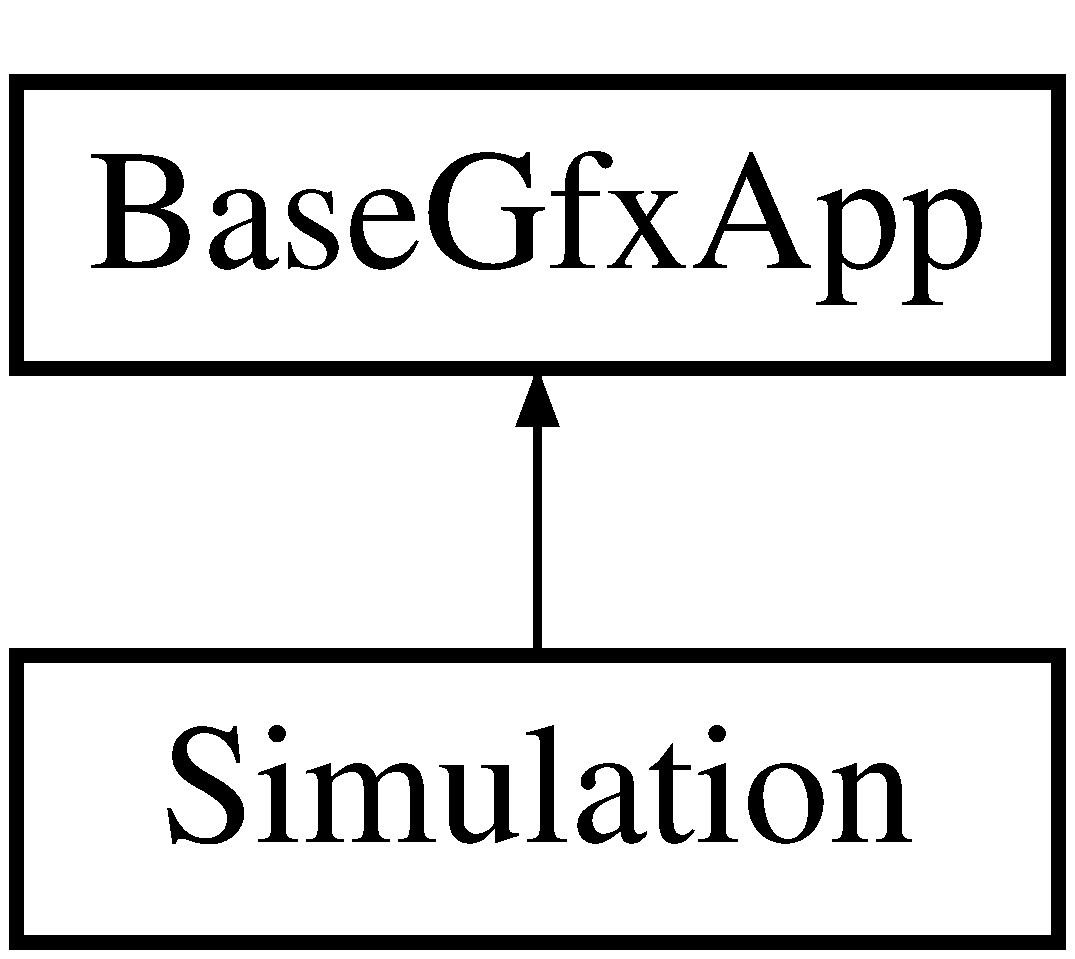
\includegraphics[height=2.000000cm]{classBaseGfxApp}
\end{center}
\end{figure}
\subsection*{Public Member Functions}
\begin{DoxyCompactItemize}
\item 
\hypertarget{classBaseGfxApp_a534a4b5293a35947fdae3805a103541d}{{\bfseries Base\-Gfx\-App} (int argc, char $\ast$argv\mbox{[}$\,$\mbox{]}, int width, int height, int x, int y, int glut\-Flags, bool create\-G\-L\-U\-I\-Win, int glui\-Win\-X, int glui\-Win\-Y)}\label{classBaseGfxApp_a534a4b5293a35947fdae3805a103541d}

\item 
\hypertarget{classBaseGfxApp_a4b3b1a475b7f2babaf1b477c34b15fb1}{void {\bfseries set\-Caption} (const std\-::string \&caption)}\label{classBaseGfxApp_a4b3b1a475b7f2babaf1b477c34b15fb1}

\item 
\hypertarget{classBaseGfxApp_acda031916c00d56c2dc901e2653e3083}{void {\bfseries run\-Main\-Loop} ()}\label{classBaseGfxApp_acda031916c00d56c2dc901e2653e3083}

\item 
\hypertarget{classBaseGfxApp_ac8de2d5a955582547af5619b771b4d6d}{virtual void {\bfseries display} ()}\label{classBaseGfxApp_ac8de2d5a955582547af5619b771b4d6d}

\item 
\hypertarget{classBaseGfxApp_a0956b82d7fa58b623c498aea7073dbba}{virtual void {\bfseries mouse\-Moved} (int x, int y)}\label{classBaseGfxApp_a0956b82d7fa58b623c498aea7073dbba}

\item 
\hypertarget{classBaseGfxApp_abb23f716dd6612b3a72938e41525d338}{virtual void {\bfseries mouse\-Dragged} (int x, int y)}\label{classBaseGfxApp_abb23f716dd6612b3a72938e41525d338}

\item 
\hypertarget{classBaseGfxApp_aaaccf5a5e923a9465441a5ee712424a8}{virtual void {\bfseries left\-Mouse\-Down} (int x, int y)}\label{classBaseGfxApp_aaaccf5a5e923a9465441a5ee712424a8}

\item 
\hypertarget{classBaseGfxApp_a0a2961a932b02b2f9d7d0bb408f6fb51}{virtual void {\bfseries left\-Mouse\-Up} (int x, int y)}\label{classBaseGfxApp_a0a2961a932b02b2f9d7d0bb408f6fb51}

\item 
\hypertarget{classBaseGfxApp_afa87e6a71220945e41f0424e540125d9}{virtual void {\bfseries right\-Mouse\-Down} (int x, int y)}\label{classBaseGfxApp_afa87e6a71220945e41f0424e540125d9}

\item 
\hypertarget{classBaseGfxApp_a812643d563522a993457dd565c33f8f6}{virtual void {\bfseries right\-Mouse\-Up} (int x, int y)}\label{classBaseGfxApp_a812643d563522a993457dd565c33f8f6}

\item 
\hypertarget{classBaseGfxApp_a2c98cae9bb5ad1fb1832a6d4812670f8}{virtual void {\bfseries middle\-Mouse\-Down} (int x, int y)}\label{classBaseGfxApp_a2c98cae9bb5ad1fb1832a6d4812670f8}

\item 
\hypertarget{classBaseGfxApp_a00fc05e8d9629b72302b5adf014bdb0c}{virtual void {\bfseries middle\-Mouse\-Up} (int x, int y)}\label{classBaseGfxApp_a00fc05e8d9629b72302b5adf014bdb0c}

\item 
\hypertarget{classBaseGfxApp_a6d91e0cb7a3d48cad33956efe7eb36ca}{virtual void {\bfseries keyboard} (unsigned char c, int x, int y)}\label{classBaseGfxApp_a6d91e0cb7a3d48cad33956efe7eb36ca}

\item 
\hypertarget{classBaseGfxApp_a345566e62c9e4ec3705ec4d1c4c75f1f}{virtual void {\bfseries keyboard\-Special} (int key, int x, int y)}\label{classBaseGfxApp_a345566e62c9e4ec3705ec4d1c4c75f1f}

\item 
\hypertarget{classBaseGfxApp_acc4a40ce11edd6b6660a19cb4802a2bf}{virtual void {\bfseries keyboard\-Up} (unsigned char c, int x, int y)}\label{classBaseGfxApp_acc4a40ce11edd6b6660a19cb4802a2bf}

\item 
\hypertarget{classBaseGfxApp_afd14b435ff93b1e7f461cb8bd1a6fd59}{virtual void {\bfseries keyboard\-Special\-Up} (int key, int x, int y)}\label{classBaseGfxApp_afd14b435ff93b1e7f461cb8bd1a6fd59}

\item 
\hypertarget{classBaseGfxApp_a5d8d5d778a8aecd7f5f8e9c87f4c3d20}{virtual void {\bfseries reshape} (int width, int height)}\label{classBaseGfxApp_a5d8d5d778a8aecd7f5f8e9c87f4c3d20}

\item 
\hypertarget{classBaseGfxApp_a2978a7c358794c67df73b66776b2cef3}{virtual void {\bfseries glui\-Control} (int control\-I\-D)}\label{classBaseGfxApp_a2978a7c358794c67df73b66776b2cef3}

\item 
\hypertarget{classBaseGfxApp_ace089a1a94fb6bb0bc17e1b7fa48e05d}{int {\bfseries width} () const }\label{classBaseGfxApp_ace089a1a94fb6bb0bc17e1b7fa48e05d}

\item 
\hypertarget{classBaseGfxApp_aa253dbe16a20c40e0a1bf8ff942ceea3}{int {\bfseries height} () const }\label{classBaseGfxApp_aa253dbe16a20c40e0a1bf8ff942ceea3}

\item 
\hypertarget{classBaseGfxApp_ae9779f948eff6f45beec08091e98a803}{int {\bfseries handle} ()}\label{classBaseGfxApp_ae9779f948eff6f45beec08091e98a803}

\item 
\hypertarget{classBaseGfxApp_ac721a0fedce80308c5c0e5695016e95d}{G\-L\-U\-I $\ast$ {\bfseries glui} ()}\label{classBaseGfxApp_ac721a0fedce80308c5c0e5695016e95d}

\end{DoxyCompactItemize}
\subsection*{Static Protected Member Functions}
\begin{DoxyCompactItemize}
\item 
\hypertarget{classBaseGfxApp_a5fe6a77d37044cbe28647ed3391bbb7a}{static void {\bfseries s\-\_\-reshape} (int width, int height)}\label{classBaseGfxApp_a5fe6a77d37044cbe28647ed3391bbb7a}

\item 
\hypertarget{classBaseGfxApp_a52edb2569227319feb68779844e7d857}{static void {\bfseries s\-\_\-keyboard} (unsigned char c, int x, int y)}\label{classBaseGfxApp_a52edb2569227319feb68779844e7d857}

\item 
\hypertarget{classBaseGfxApp_a1e8d90a4faab60300ddf2a4ea9b83115}{static void {\bfseries s\-\_\-keyboardspecial} (int key, int x, int y)}\label{classBaseGfxApp_a1e8d90a4faab60300ddf2a4ea9b83115}

\item 
\hypertarget{classBaseGfxApp_aa1ca205af9d6cee33949f2e6adf4c923}{static void {\bfseries s\-\_\-keyboardup} (unsigned char c, int x, int y)}\label{classBaseGfxApp_aa1ca205af9d6cee33949f2e6adf4c923}

\item 
\hypertarget{classBaseGfxApp_a0e4dfe006f3cc9126c1cc8ad32784f75}{static void {\bfseries s\-\_\-keyboardspecialup} (int key, int x, int y)}\label{classBaseGfxApp_a0e4dfe006f3cc9126c1cc8ad32784f75}

\item 
\hypertarget{classBaseGfxApp_a5e640f2394f7e038d0dd2b469d5c2e24}{static void {\bfseries s\-\_\-mousemotion} (int x, int y)}\label{classBaseGfxApp_a5e640f2394f7e038d0dd2b469d5c2e24}

\item 
\hypertarget{classBaseGfxApp_a22dd953bfb75add9fd0f8f2f8be535c5}{static void {\bfseries s\-\_\-mousebtn} (int b, int s, int x, int y)}\label{classBaseGfxApp_a22dd953bfb75add9fd0f8f2f8be535c5}

\item 
\hypertarget{classBaseGfxApp_a58415c6151a2a80e1fe2eaa9919a4dab}{static void {\bfseries s\-\_\-draw} ()}\label{classBaseGfxApp_a58415c6151a2a80e1fe2eaa9919a4dab}

\item 
\hypertarget{classBaseGfxApp_ad4a963321f1147d68369225ab0c7f32f}{static void {\bfseries s\-\_\-gluicallback} (int control\-I\-D)}\label{classBaseGfxApp_ad4a963321f1147d68369225ab0c7f32f}

\end{DoxyCompactItemize}
\subsection*{Protected Attributes}
\begin{DoxyCompactItemize}
\item 
int \hyperlink{classBaseGfxApp_ad8697d6fdd10e6f336c3a662016b4fa7}{m\-\_\-glut\-Window\-Handle}
\item 
\hypertarget{classBaseGfxApp_a6eb1673b80283727221da2242211af1d}{G\-L\-U\-I $\ast$ {\bfseries m\-\_\-glui}}\label{classBaseGfxApp_a6eb1673b80283727221da2242211af1d}

\item 
\hypertarget{classBaseGfxApp_a2e70a389224f8affe7c137f7e20dc8c1}{bool {\bfseries m\-\_\-drag}}\label{classBaseGfxApp_a2e70a389224f8affe7c137f7e20dc8c1}

\item 
\hypertarget{classBaseGfxApp_a7e5ef1c8f25fe081b4a1fd4ce6a96e07}{int {\bfseries m\-\_\-width}}\label{classBaseGfxApp_a7e5ef1c8f25fe081b4a1fd4ce6a96e07}

\item 
\hypertarget{classBaseGfxApp_ac078e4fc20b5c2fe0c744966b850b412}{int {\bfseries m\-\_\-height}}\label{classBaseGfxApp_ac078e4fc20b5c2fe0c744966b850b412}

\end{DoxyCompactItemize}
\subsection*{Static Protected Attributes}
\begin{DoxyCompactItemize}
\item 
static \hyperlink{classBaseGfxApp}{Base\-Gfx\-App} $\ast$ \hyperlink{classBaseGfxApp_a65ba89b98af31e2649a0546631931000}{s\-\_\-current\-App} = N\-U\-L\-L
\item 
static bool \hyperlink{classBaseGfxApp_afa4690383ea27713016ef75b9fb1e42f}{s\-\_\-glut\-Initialized} = false
\end{DoxyCompactItemize}


\subsection{Member Data Documentation}
\hypertarget{classBaseGfxApp_ad8697d6fdd10e6f336c3a662016b4fa7}{\index{Base\-Gfx\-App@{Base\-Gfx\-App}!m\-\_\-glut\-Window\-Handle@{m\-\_\-glut\-Window\-Handle}}
\index{m\-\_\-glut\-Window\-Handle@{m\-\_\-glut\-Window\-Handle}!BaseGfxApp@{Base\-Gfx\-App}}
\subsubsection[{m\-\_\-glut\-Window\-Handle}]{\setlength{\rightskip}{0pt plus 5cm}int Base\-Gfx\-App\-::m\-\_\-glut\-Window\-Handle\hspace{0.3cm}{\ttfamily [protected]}}}\label{classBaseGfxApp_ad8697d6fdd10e6f336c3a662016b4fa7}
Underlying glut window handle \hypertarget{classBaseGfxApp_a65ba89b98af31e2649a0546631931000}{\index{Base\-Gfx\-App@{Base\-Gfx\-App}!s\-\_\-current\-App@{s\-\_\-current\-App}}
\index{s\-\_\-current\-App@{s\-\_\-current\-App}!BaseGfxApp@{Base\-Gfx\-App}}
\subsubsection[{s\-\_\-current\-App}]{\setlength{\rightskip}{0pt plus 5cm}{\bf Base\-Gfx\-App} $\ast$ Base\-Gfx\-App\-::s\-\_\-current\-App = N\-U\-L\-L\hspace{0.3cm}{\ttfamily [static]}, {\ttfamily [protected]}}}\label{classBaseGfxApp_a65ba89b98af31e2649a0546631931000}
G\-L\-U\-T and G\-L\-U\-I event callbacks are sent to the current window/app. Right now, there is only one window anyway (not counting the G\-L\-U\-I U\-I window.. in the future could be extended to support more windows. In any case, some structure like this is always needed when using glut with C++, since the glut callbacks must be either global or static functions. \hypertarget{classBaseGfxApp_afa4690383ea27713016ef75b9fb1e42f}{\index{Base\-Gfx\-App@{Base\-Gfx\-App}!s\-\_\-glut\-Initialized@{s\-\_\-glut\-Initialized}}
\index{s\-\_\-glut\-Initialized@{s\-\_\-glut\-Initialized}!BaseGfxApp@{Base\-Gfx\-App}}
\subsubsection[{s\-\_\-glut\-Initialized}]{\setlength{\rightskip}{0pt plus 5cm}bool Base\-Gfx\-App\-::s\-\_\-glut\-Initialized = false\hspace{0.3cm}{\ttfamily [static]}, {\ttfamily [protected]}}}\label{classBaseGfxApp_afa4690383ea27713016ef75b9fb1e42f}
Has glut\-Init been called? (only allowed once per program) 

The documentation for this class was generated from the following files\-:\begin{DoxyCompactItemize}
\item 
\hyperlink{BaseGfxApp_8hpp}{Base\-Gfx\-App.\-hpp}\item 
Base\-Gfx\-App.\-cpp\end{DoxyCompactItemize}

\hypertarget{classBaseObject}{\section{Base\-Object Class Reference}
\label{classBaseObject}\index{Base\-Object@{Base\-Object}}
}
Inheritance diagram for Base\-Object\-:\begin{figure}[H]
\begin{center}
\leavevmode
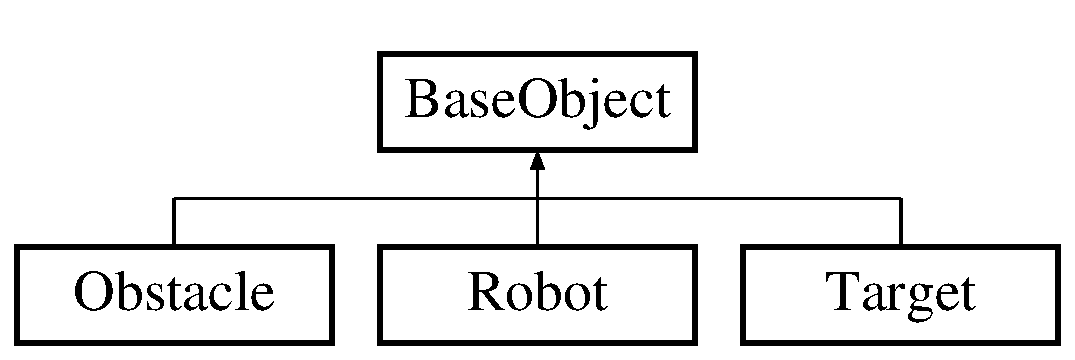
\includegraphics[height=2.000000cm]{classBaseObject}
\end{center}
\end{figure}
\subsection*{Public Member Functions}
\begin{DoxyCompactItemize}
\item 
\hyperlink{classBaseObject_ae6fa65bf33f26d46a6aa1a5ef9ee63c9}{Base\-Object} (char type, int speed\-Rating)
\item 
\hyperlink{classBaseObject_ababc1565c1eb8038f6c85886b9c3781c}{Base\-Object} (char type, int speed\-Rating, int size\-Rating)
\item 
\hyperlink{classBaseObject_a83eecfd3bdaffda4e6c7d0fb98747f96}{$\sim$\-Base\-Object} ()
\item 
int \hyperlink{classBaseObject_a6d4bd3f6a445bf8f4c304582e5a8c71d}{get\-I\-D} () const 
\item 
char \hyperlink{classBaseObject_ab333e5027b28d1dbe97736297efd1b94}{get\-Type} () const 
\item 
int \hyperlink{classBaseObject_a6dc634df2e679f28ab1435d494a3375e}{get\-Radius} () const 
\item 
int \hyperlink{classBaseObject_ac46f29b5be2bc1036115e5ee76f3996f}{get\-Speed} () const 
\item 
std\-::pair$<$ int, int $>$ \hyperlink{classBaseObject_a85cace89c6a85cb8e312e6e8a1decf29}{get\-Colors} () const 
\item 
void \hyperlink{classBaseObject_ad983298291c7600a244caebedd25bdfc}{set\-I\-D} (int id)
\item 
void \hyperlink{classBaseObject_a97b5625fa993c44e523f6f7be4230b4b}{set\-Type} (char type)
\item 
void \hyperlink{classBaseObject_a4157e3766c87cf1cda114a6239e1298c}{set\-Radius} (int radius)
\item 
void \hyperlink{classBaseObject_a662c7c9fd38d0dcfc102c737a0dbc5f8}{set\-Random\-Radius} ()
\item 
void \hyperlink{classBaseObject_a968935f7fc333e5ed67f7cbfe526720b}{set\-Speed} (int speed\-Rating)
\item 
void \hyperlink{classBaseObject_a33b50bfd5a5be9b504194aeadecc5e1e}{set\-Colors} (int primary, int secondary)
\item 
void \hyperlink{classBaseObject_ab89fb453f3e974db33f131bcce4559d6}{set\-Flags} (std\-::vector$<$ std\-::pair$<$ int, char $>$ $>$ colliding\-Objs)
\item 
\hypertarget{classBaseObject_a8608698c308c58ebf3a7f03541556b05}{virtual void {\bfseries sensor\-Scans} ()}\label{classBaseObject_a8608698c308c58ebf3a7f03541556b05}

\item 
\hypertarget{classBaseObject_a74591ce3c625f36937d43040557937f6}{virtual std\-::pair$<$ int, int $>$ {\bfseries move} (int elapsed\-Time)=0}\label{classBaseObject_a74591ce3c625f36937d43040557937f6}

\end{DoxyCompactItemize}
\subsection*{Static Public Member Functions}
\begin{DoxyCompactItemize}
\item 
static \hyperlink{classEnvironment}{Environment} $\ast$ \hyperlink{classBaseObject_a3f3c53a54006151370013c39262682c6}{get\-Env} ()
\end{DoxyCompactItemize}
\subsection*{Protected Member Functions}
\begin{DoxyCompactItemize}
\item 
void \hyperlink{classBaseObject_ad202362d71b6e41b168e88592c5c5fc0}{reset\-Flags} ()
\end{DoxyCompactItemize}
\subsection*{Protected Attributes}
\begin{DoxyCompactItemize}
\item 
\hypertarget{classBaseObject_ab21889ef86ffc1849898d2613ccdc75f}{int {\bfseries id}}\label{classBaseObject_ab21889ef86ffc1849898d2613ccdc75f}

\item 
\hypertarget{classBaseObject_a4bd0bd6f8e263af7621ec80b47ebbad1}{int {\bfseries radius}}\label{classBaseObject_a4bd0bd6f8e263af7621ec80b47ebbad1}

\item 
\hypertarget{classBaseObject_a77eb913a6f92fc275fdcc679d2377ed8}{int {\bfseries speed}}\label{classBaseObject_a77eb913a6f92fc275fdcc679d2377ed8}

\item 
\hypertarget{classBaseObject_acde20ad83b864b997b2e81b29303d25b}{char {\bfseries type}}\label{classBaseObject_acde20ad83b864b997b2e81b29303d25b}

\item 
\hypertarget{classBaseObject_a4e59f6ee35255ef92325f0edcd849e25}{std\-::pair$<$ int, int $>$ {\bfseries colors}}\label{classBaseObject_a4e59f6ee35255ef92325f0edcd849e25}

\item 
\hypertarget{classBaseObject_a16bede1971c3e62957ca033fd521ca8b}{bool {\bfseries collide\-Wall}}\label{classBaseObject_a16bede1971c3e62957ca033fd521ca8b}

\item 
\hypertarget{classBaseObject_ad22a16beb1d41db1107bef67e2346583}{bool {\bfseries collide\-Robot}}\label{classBaseObject_ad22a16beb1d41db1107bef67e2346583}

\item 
\hypertarget{classBaseObject_a7439c5dfdc2078ecccaaf820b3b0f521}{bool {\bfseries collide\-Obstacle}}\label{classBaseObject_a7439c5dfdc2078ecccaaf820b3b0f521}

\item 
\hypertarget{classBaseObject_a9ac15037c8c2b321eb746957306d43f2}{bool {\bfseries collide\-Target}}\label{classBaseObject_a9ac15037c8c2b321eb746957306d43f2}

\end{DoxyCompactItemize}
\subsection*{Static Protected Attributes}
\begin{DoxyCompactItemize}
\item 
static \hyperlink{classEnvironment}{Environment} $\ast$ \hyperlink{classBaseObject_adf47773f2b71699caa9560be64ccfbbe}{env}
\end{DoxyCompactItemize}


\subsection{Constructor \& Destructor Documentation}
\hypertarget{classBaseObject_ae6fa65bf33f26d46a6aa1a5ef9ee63c9}{\index{Base\-Object@{Base\-Object}!Base\-Object@{Base\-Object}}
\index{Base\-Object@{Base\-Object}!BaseObject@{Base\-Object}}
\subsubsection[{Base\-Object}]{\setlength{\rightskip}{0pt plus 5cm}Base\-Object\-::\-Base\-Object (
\begin{DoxyParamCaption}
\item[{char}]{type, }
\item[{int}]{speed\-Rating}
\end{DoxyParamCaption}
)}}\label{classBaseObject_ae6fa65bf33f26d46a6aa1a5ef9ee63c9}
Constructor for the physical objects, which are parents of the other derived types. sets the object with a random speed. \hypertarget{classBaseObject_ababc1565c1eb8038f6c85886b9c3781c}{\index{Base\-Object@{Base\-Object}!Base\-Object@{Base\-Object}}
\index{Base\-Object@{Base\-Object}!BaseObject@{Base\-Object}}
\subsubsection[{Base\-Object}]{\setlength{\rightskip}{0pt plus 5cm}Base\-Object\-::\-Base\-Object (
\begin{DoxyParamCaption}
\item[{char}]{type, }
\item[{int}]{speed\-Rating, }
\item[{int}]{size\-Rating}
\end{DoxyParamCaption}
)}}\label{classBaseObject_ababc1565c1eb8038f6c85886b9c3781c}
Constructor for physical objects, which are parents of other derived types. \hypertarget{classBaseObject_a83eecfd3bdaffda4e6c7d0fb98747f96}{\index{Base\-Object@{Base\-Object}!$\sim$\-Base\-Object@{$\sim$\-Base\-Object}}
\index{$\sim$\-Base\-Object@{$\sim$\-Base\-Object}!BaseObject@{Base\-Object}}
\subsubsection[{$\sim$\-Base\-Object}]{\setlength{\rightskip}{0pt plus 5cm}Base\-Object\-::$\sim$\-Base\-Object (
\begin{DoxyParamCaption}
{}
\end{DoxyParamCaption}
)}}\label{classBaseObject_a83eecfd3bdaffda4e6c7d0fb98747f96}
Destructor 

\subsection{Member Function Documentation}
\hypertarget{classBaseObject_a85cace89c6a85cb8e312e6e8a1decf29}{\index{Base\-Object@{Base\-Object}!get\-Colors@{get\-Colors}}
\index{get\-Colors@{get\-Colors}!BaseObject@{Base\-Object}}
\subsubsection[{get\-Colors}]{\setlength{\rightskip}{0pt plus 5cm}std\-::pair$<$ int, int $>$ Base\-Object\-::get\-Colors (
\begin{DoxyParamCaption}
{}
\end{DoxyParamCaption}
) const}}\label{classBaseObject_a85cace89c6a85cb8e312e6e8a1decf29}
method which returns the primary and secondary colors of the object \hypertarget{classBaseObject_a3f3c53a54006151370013c39262682c6}{\index{Base\-Object@{Base\-Object}!get\-Env@{get\-Env}}
\index{get\-Env@{get\-Env}!BaseObject@{Base\-Object}}
\subsubsection[{get\-Env}]{\setlength{\rightskip}{0pt plus 5cm}{\bf Environment} $\ast$ Base\-Object\-::get\-Env (
\begin{DoxyParamCaption}
{}
\end{DoxyParamCaption}
)\hspace{0.3cm}{\ttfamily [static]}}}\label{classBaseObject_a3f3c53a54006151370013c39262682c6}
Method which returns a pointer to the static environment member variable \hypertarget{classBaseObject_a6d4bd3f6a445bf8f4c304582e5a8c71d}{\index{Base\-Object@{Base\-Object}!get\-I\-D@{get\-I\-D}}
\index{get\-I\-D@{get\-I\-D}!BaseObject@{Base\-Object}}
\subsubsection[{get\-I\-D}]{\setlength{\rightskip}{0pt plus 5cm}int Base\-Object\-::get\-I\-D (
\begin{DoxyParamCaption}
{}
\end{DoxyParamCaption}
) const}}\label{classBaseObject_a6d4bd3f6a445bf8f4c304582e5a8c71d}
Method which returns the id of the object \hypertarget{classBaseObject_a6dc634df2e679f28ab1435d494a3375e}{\index{Base\-Object@{Base\-Object}!get\-Radius@{get\-Radius}}
\index{get\-Radius@{get\-Radius}!BaseObject@{Base\-Object}}
\subsubsection[{get\-Radius}]{\setlength{\rightskip}{0pt plus 5cm}int Base\-Object\-::get\-Radius (
\begin{DoxyParamCaption}
{}
\end{DoxyParamCaption}
) const}}\label{classBaseObject_a6dc634df2e679f28ab1435d494a3375e}
Method which returns the radius of the object \hypertarget{classBaseObject_ac46f29b5be2bc1036115e5ee76f3996f}{\index{Base\-Object@{Base\-Object}!get\-Speed@{get\-Speed}}
\index{get\-Speed@{get\-Speed}!BaseObject@{Base\-Object}}
\subsubsection[{get\-Speed}]{\setlength{\rightskip}{0pt plus 5cm}int Base\-Object\-::get\-Speed (
\begin{DoxyParamCaption}
{}
\end{DoxyParamCaption}
) const}}\label{classBaseObject_ac46f29b5be2bc1036115e5ee76f3996f}
Method which returns the speed of the object \hypertarget{classBaseObject_ab333e5027b28d1dbe97736297efd1b94}{\index{Base\-Object@{Base\-Object}!get\-Type@{get\-Type}}
\index{get\-Type@{get\-Type}!BaseObject@{Base\-Object}}
\subsubsection[{get\-Type}]{\setlength{\rightskip}{0pt plus 5cm}char Base\-Object\-::get\-Type (
\begin{DoxyParamCaption}
{}
\end{DoxyParamCaption}
) const}}\label{classBaseObject_ab333e5027b28d1dbe97736297efd1b94}
Method which returns the type of the object \hypertarget{classBaseObject_ad202362d71b6e41b168e88592c5c5fc0}{\index{Base\-Object@{Base\-Object}!reset\-Flags@{reset\-Flags}}
\index{reset\-Flags@{reset\-Flags}!BaseObject@{Base\-Object}}
\subsubsection[{reset\-Flags}]{\setlength{\rightskip}{0pt plus 5cm}void Base\-Object\-::reset\-Flags (
\begin{DoxyParamCaption}
{}
\end{DoxyParamCaption}
)\hspace{0.3cm}{\ttfamily [protected]}}}\label{classBaseObject_ad202362d71b6e41b168e88592c5c5fc0}
Method which resets all collision flags to false \hypertarget{classBaseObject_a33b50bfd5a5be9b504194aeadecc5e1e}{\index{Base\-Object@{Base\-Object}!set\-Colors@{set\-Colors}}
\index{set\-Colors@{set\-Colors}!BaseObject@{Base\-Object}}
\subsubsection[{set\-Colors}]{\setlength{\rightskip}{0pt plus 5cm}void Base\-Object\-::set\-Colors (
\begin{DoxyParamCaption}
\item[{int}]{primary, }
\item[{int}]{secondary}
\end{DoxyParamCaption}
)}}\label{classBaseObject_a33b50bfd5a5be9b504194aeadecc5e1e}
Method which sets the primary and secondary colors of the object. Note that these values are simply set to integers. only the graphics display cares about actual colors. In this scope integers are sufficient since all that matters is that objects with different colors are drawn differently \hypertarget{classBaseObject_ab89fb453f3e974db33f131bcce4559d6}{\index{Base\-Object@{Base\-Object}!set\-Flags@{set\-Flags}}
\index{set\-Flags@{set\-Flags}!BaseObject@{Base\-Object}}
\subsubsection[{set\-Flags}]{\setlength{\rightskip}{0pt plus 5cm}void Base\-Object\-::set\-Flags (
\begin{DoxyParamCaption}
\item[{std\-::vector$<$ std\-::pair$<$ int, char $>$ $>$}]{colliding\-Objs}
\end{DoxyParamCaption}
)}}\label{classBaseObject_ab89fb453f3e974db33f131bcce4559d6}
Method which sets flags based on current collision values \hypertarget{classBaseObject_ad983298291c7600a244caebedd25bdfc}{\index{Base\-Object@{Base\-Object}!set\-I\-D@{set\-I\-D}}
\index{set\-I\-D@{set\-I\-D}!BaseObject@{Base\-Object}}
\subsubsection[{set\-I\-D}]{\setlength{\rightskip}{0pt plus 5cm}void Base\-Object\-::set\-I\-D (
\begin{DoxyParamCaption}
\item[{int}]{id}
\end{DoxyParamCaption}
)}}\label{classBaseObject_ad983298291c7600a244caebedd25bdfc}
Sets the object I\-D \hypertarget{classBaseObject_a4157e3766c87cf1cda114a6239e1298c}{\index{Base\-Object@{Base\-Object}!set\-Radius@{set\-Radius}}
\index{set\-Radius@{set\-Radius}!BaseObject@{Base\-Object}}
\subsubsection[{set\-Radius}]{\setlength{\rightskip}{0pt plus 5cm}void Base\-Object\-::set\-Radius (
\begin{DoxyParamCaption}
\item[{int}]{size\-Rating}
\end{DoxyParamCaption}
)}}\label{classBaseObject_a4157e3766c87cf1cda114a6239e1298c}
Method which sets the radius of the object based on a size rating from 0 to 100 \hypertarget{classBaseObject_a662c7c9fd38d0dcfc102c737a0dbc5f8}{\index{Base\-Object@{Base\-Object}!set\-Random\-Radius@{set\-Random\-Radius}}
\index{set\-Random\-Radius@{set\-Random\-Radius}!BaseObject@{Base\-Object}}
\subsubsection[{set\-Random\-Radius}]{\setlength{\rightskip}{0pt plus 5cm}void Base\-Object\-::set\-Random\-Radius (
\begin{DoxyParamCaption}
{}
\end{DoxyParamCaption}
)}}\label{classBaseObject_a662c7c9fd38d0dcfc102c737a0dbc5f8}
Method which computes a random size rating and sets the object radius accordingly \hypertarget{classBaseObject_a968935f7fc333e5ed67f7cbfe526720b}{\index{Base\-Object@{Base\-Object}!set\-Speed@{set\-Speed}}
\index{set\-Speed@{set\-Speed}!BaseObject@{Base\-Object}}
\subsubsection[{set\-Speed}]{\setlength{\rightskip}{0pt plus 5cm}void Base\-Object\-::set\-Speed (
\begin{DoxyParamCaption}
\item[{int}]{speed\-Rating}
\end{DoxyParamCaption}
)}}\label{classBaseObject_a968935f7fc333e5ed67f7cbfe526720b}
Method which sets the speed of the object based on a speed rating between 0 and 100 \hypertarget{classBaseObject_a97b5625fa993c44e523f6f7be4230b4b}{\index{Base\-Object@{Base\-Object}!set\-Type@{set\-Type}}
\index{set\-Type@{set\-Type}!BaseObject@{Base\-Object}}
\subsubsection[{set\-Type}]{\setlength{\rightskip}{0pt plus 5cm}void Base\-Object\-::set\-Type (
\begin{DoxyParamCaption}
\item[{char}]{type}
\end{DoxyParamCaption}
)}}\label{classBaseObject_a97b5625fa993c44e523f6f7be4230b4b}
Method which returns the type of the object. 'r' for robot, 'o' for obstacle, 't' for target 

\subsection{Member Data Documentation}
\hypertarget{classBaseObject_adf47773f2b71699caa9560be64ccfbbe}{\index{Base\-Object@{Base\-Object}!env@{env}}
\index{env@{env}!BaseObject@{Base\-Object}}
\subsubsection[{env}]{\setlength{\rightskip}{0pt plus 5cm}{\bf Environment} $\ast$ Base\-Object\-::env\hspace{0.3cm}{\ttfamily [static]}, {\ttfamily [protected]}}}\label{classBaseObject_adf47773f2b71699caa9560be64ccfbbe}
Defining the static env member variable 

The documentation for this class was generated from the following files\-:\begin{DoxyCompactItemize}
\item 
\hyperlink{BaseObject_8hpp}{Base\-Object.\-hpp}\item 
Base\-Object.\-cpp\end{DoxyCompactItemize}

\hypertarget{classEnvironment}{\section{Environment Class Reference}
\label{classEnvironment}\index{Environment@{Environment}}
}


{\ttfamily \#include $<$Environment.\-hpp$>$}

\subsection*{Public Types}
\begin{DoxyCompactItemize}
\item 
typedef std\-::vector$<$ std\-::pair\\*
$<$ int, char $>$ $>$ \hyperlink{classEnvironment_a9609fedf5c7244c3515c8e5640b81e85}{Collide\-Vector\-Pair}
\item 
typedef std\-::pair$<$ int, int $>$ \hyperlink{classEnvironment_aa0cae1577b893c94479b544518c11d3b}{Homing\-Pair}
\end{DoxyCompactItemize}
\subsection*{Public Member Functions}
\begin{DoxyCompactItemize}
\item 
\hyperlink{classEnvironment_a005e7ffe869ab060891880d058407ae0}{Environment} (const int width, const int height, const int scale\-Factor)
\item 
\hyperlink{classEnvironment_a8e294735187880dd3d59be10c425b29d}{$\sim$\-Environment} ()
\item 
\hyperlink{classWalls}{Walls} $\ast$ \hyperlink{classEnvironment_aeb10b316d1a388fa633613d5a7c1c095}{get\-Walls} () const 
\item 
char \hyperlink{classEnvironment_a40f36635e3a08093bfc7c13dae1ab802}{get\-Object\-Type} (const int index) const 
\item 
std\-::pair$<$ int, int $>$ \hyperlink{classEnvironment_a21de28a8d647dd3dfa097faaa76266c8}{get\-Object\-Position} (const int index) const 
\item 
int \hyperlink{classEnvironment_a57407c2a4127023ab3e3e8631d742b45}{get\-Object\-Orientation} (const int index) const 
\item 
int \hyperlink{classEnvironment_ab09800efb10e10230b8f49dbea0c4019}{get\-Object\-Radius} (const int index) const 
\item 
std\-::pair$<$ int, int $>$ \hyperlink{classEnvironment_ad233a196b5e2d3d9a21194011d135335}{get\-Object\-Colors} (const int index) const 
\item 
bool \hyperlink{classEnvironment_a3bae68ad481d5c6da8846ffed6ec08fc}{get\-Object\-Obstacle\-Collision\-Status} (const int index) const 
\item 
int \hyperlink{classEnvironment_a9808cd4199ace6e21de16b2e37ed4212}{get\-Num\-Objects} () const 
\item 
int \hyperlink{classEnvironment_ac5ad865f384d0c4656a76c8e44f77441}{register\-Object} (\hyperlink{classBaseObject}{Base\-Object} $\ast$obj\-Ptr)
\item 
void \hyperlink{classEnvironment_a25ab88a722c206c100eba3a5788d88c4}{update} (int elapsed\-Time)
\item 
\hyperlink{classEnvironment_a9609fedf5c7244c3515c8e5640b81e85}{Collide\-Vector\-Pair} \hyperlink{classEnvironment_acd2595742e8d30962d90d6871a184ba6}{touch\-Sensor\-Reading} (int obj\-I\-D)
\item 
\hyperlink{classEnvironment_aa0cae1577b893c94479b544518c11d3b}{Homing\-Pair} \hyperlink{classEnvironment_a681b85535a9a7dbc2b594d28d6c61e81}{homing\-Sensor\-Reading} (int robot\-I\-D)
\end{DoxyCompactItemize}


\subsection{Detailed Description}
\hyperlink{classEnvironment}{Environment} Class means to store physical object and register Object. Rendering and \hyperlink{classBaseObject}{Base\-Object} inherit from this class. 

\subsection{Member Typedef Documentation}
\hypertarget{classEnvironment_a9609fedf5c7244c3515c8e5640b81e85}{\index{Environment@{Environment}!Collide\-Vector\-Pair@{Collide\-Vector\-Pair}}
\index{Collide\-Vector\-Pair@{Collide\-Vector\-Pair}!Environment@{Environment}}
\subsubsection[{Collide\-Vector\-Pair}]{\setlength{\rightskip}{0pt plus 5cm}typedef std\-::vector$<$ std\-::pair$<$int,char$>$ $>$ {\bf Environment\-::\-Collide\-Vector\-Pair}}}\label{classEnvironment_a9609fedf5c7244c3515c8e5640b81e85}
Colliding anything with the environment. Storing the position and radius about the current object. For colliding Objects are stored in some hidden data structure. Colliding object can be changing continuously because of random. Accordingly to change I\-D. An internal data structure is set up to store information about object collision status Checking I\-D and the robot is overlapping the wall or antoehr object. A pointer to the colliding object is passed to this function An internal data structure store colliding information. \hypertarget{classEnvironment_aa0cae1577b893c94479b544518c11d3b}{\index{Environment@{Environment}!Homing\-Pair@{Homing\-Pair}}
\index{Homing\-Pair@{Homing\-Pair}!Environment@{Environment}}
\subsubsection[{Homing\-Pair}]{\setlength{\rightskip}{0pt plus 5cm}typedef std\-::pair$<$int,int$>$ {\bf Environment\-::\-Homing\-Pair}}}\label{classEnvironment_aa0cae1577b893c94479b544518c11d3b}
Homing the target with the environment. The amount must rotate and move forward to reach the target. Checking the target position and the robot position. Calculating the theta using math.\-atan2. Don't caring about negative. Making target\-Angel\-Offset. Also, calculate the distance between target and robot. Return distance and direction from target. 

\subsection{Constructor \& Destructor Documentation}
\hypertarget{classEnvironment_a005e7ffe869ab060891880d058407ae0}{\index{Environment@{Environment}!Environment@{Environment}}
\index{Environment@{Environment}!Environment@{Environment}}
\subsubsection[{Environment}]{\setlength{\rightskip}{0pt plus 5cm}Environment\-::\-Environment (
\begin{DoxyParamCaption}
\item[{const int}]{width, }
\item[{const int}]{height, }
\item[{const int}]{scale\-Factor}
\end{DoxyParamCaption}
)}}\label{classEnvironment_a005e7ffe869ab060891880d058407ae0}
The constructor for an \hyperlink{classEnvironment}{Environment}. This class takes two arguments, the width and height of the environment 
\begin{DoxyParams}{Parameters}
{\em width} & The wall dimension A poiter is the area of movable to target or object. \\
\hline
{\em height} & The wall dimension A vector of objects keep track of other objects that are also currently being displayed.\\
\hline
\end{DoxyParams}
Constructor for \hyperlink{classEnvironment}{Environment} takes two arguments, the width and height of the environment Constructing walls with given environment dimensions

Setting the numbers of robots, targets, and obstacles in the env

Creating and registering the obstacles

Creating and registering the targets

Creating and registering the robots \hypertarget{classEnvironment_a8e294735187880dd3d59be10c425b29d}{\index{Environment@{Environment}!$\sim$\-Environment@{$\sim$\-Environment}}
\index{$\sim$\-Environment@{$\sim$\-Environment}!Environment@{Environment}}
\subsubsection[{$\sim$\-Environment}]{\setlength{\rightskip}{0pt plus 5cm}Environment\-::$\sim$\-Environment (
\begin{DoxyParamCaption}
{}
\end{DoxyParamCaption}
)}}\label{classEnvironment_a8e294735187880dd3d59be10c425b29d}
The destructor for \hyperlink{classEnvironment}{Environment}. \hyperlink{classEnvironment}{Environment} free from memory.

Destructor for the \hyperlink{classEnvironment}{Environment} 

\subsection{Member Function Documentation}
\hypertarget{classEnvironment_a9808cd4199ace6e21de16b2e37ed4212}{\index{Environment@{Environment}!get\-Num\-Objects@{get\-Num\-Objects}}
\index{get\-Num\-Objects@{get\-Num\-Objects}!Environment@{Environment}}
\subsubsection[{get\-Num\-Objects}]{\setlength{\rightskip}{0pt plus 5cm}int Environment\-::get\-Num\-Objects (
\begin{DoxyParamCaption}
{}
\end{DoxyParamCaption}
) const}}\label{classEnvironment_a9808cd4199ace6e21de16b2e37ed4212}
Returns the number of objects registered with the environment \hypertarget{classEnvironment_ad233a196b5e2d3d9a21194011d135335}{\index{Environment@{Environment}!get\-Object\-Colors@{get\-Object\-Colors}}
\index{get\-Object\-Colors@{get\-Object\-Colors}!Environment@{Environment}}
\subsubsection[{get\-Object\-Colors}]{\setlength{\rightskip}{0pt plus 5cm}std\-::pair$<$ int, int $>$ Environment\-::get\-Object\-Colors (
\begin{DoxyParamCaption}
\item[{const int}]{index}
\end{DoxyParamCaption}
) const}}\label{classEnvironment_ad233a196b5e2d3d9a21194011d135335}
Returns the color of a particular object. Objects are stored in first data structure. This method accesses the objects by index in that data structure.

Returns the color of a particular object. Objects are stored in first data structure. This method accesses the objects by index in that data structure \hypertarget{classEnvironment_a3bae68ad481d5c6da8846ffed6ec08fc}{\index{Environment@{Environment}!get\-Object\-Obstacle\-Collision\-Status@{get\-Object\-Obstacle\-Collision\-Status}}
\index{get\-Object\-Obstacle\-Collision\-Status@{get\-Object\-Obstacle\-Collision\-Status}!Environment@{Environment}}
\subsubsection[{get\-Object\-Obstacle\-Collision\-Status}]{\setlength{\rightskip}{0pt plus 5cm}bool Environment\-::get\-Object\-Obstacle\-Collision\-Status (
\begin{DoxyParamCaption}
\item[{const int}]{index}
\end{DoxyParamCaption}
) const}}\label{classEnvironment_a3bae68ad481d5c6da8846ffed6ec08fc}
Finding collisions with obstacles. Returns true if \hyperlink{classObstacle}{Obstacle} is colliding with a wall, target, or object. returns false otherwise.

Returns the obstacle collision status of a particular object. Objects are stored in some hidden data structure. This method accesses the objects by index in that data structure \hypertarget{classEnvironment_a57407c2a4127023ab3e3e8631d742b45}{\index{Environment@{Environment}!get\-Object\-Orientation@{get\-Object\-Orientation}}
\index{get\-Object\-Orientation@{get\-Object\-Orientation}!Environment@{Environment}}
\subsubsection[{get\-Object\-Orientation}]{\setlength{\rightskip}{0pt plus 5cm}int Environment\-::get\-Object\-Orientation (
\begin{DoxyParamCaption}
\item[{const int}]{index}
\end{DoxyParamCaption}
) const}}\label{classEnvironment_a57407c2a4127023ab3e3e8631d742b45}
Returns the angle of orientation of a particular object. Objects are stored in second data structure. This method accesses the objects by index in that data structure.

Returns the angle of orientation of a particular object. Objects are stored in some hidden data structure. This method accesses the objects by index in that data structure \hypertarget{classEnvironment_a21de28a8d647dd3dfa097faaa76266c8}{\index{Environment@{Environment}!get\-Object\-Position@{get\-Object\-Position}}
\index{get\-Object\-Position@{get\-Object\-Position}!Environment@{Environment}}
\subsubsection[{get\-Object\-Position}]{\setlength{\rightskip}{0pt plus 5cm}std\-::pair$<$ int, int $>$ Environment\-::get\-Object\-Position (
\begin{DoxyParamCaption}
\item[{const int}]{index}
\end{DoxyParamCaption}
) const}}\label{classEnvironment_a21de28a8d647dd3dfa097faaa76266c8}
Returns the position of a particular X,Y Position obejct. Objects are stored in second data structure as pairing. This method accesses the objects by index in that data structure.

Returns the position of a particular object(\-X,\-Y). Objects are stored in some hidden data structure. This method accesses the objects by index in that data structure \hypertarget{classEnvironment_ab09800efb10e10230b8f49dbea0c4019}{\index{Environment@{Environment}!get\-Object\-Radius@{get\-Object\-Radius}}
\index{get\-Object\-Radius@{get\-Object\-Radius}!Environment@{Environment}}
\subsubsection[{get\-Object\-Radius}]{\setlength{\rightskip}{0pt plus 5cm}int Environment\-::get\-Object\-Radius (
\begin{DoxyParamCaption}
\item[{const int}]{index}
\end{DoxyParamCaption}
) const}}\label{classEnvironment_ab09800efb10e10230b8f49dbea0c4019}
Returns the radius of a particular object. Objects are stored in second data structure. This method accesses the objects by index in that data structure.

Returns the radius of a particular object. Objects are stored in some hidden data structure. This method accesses the objects by index in that data structure \hypertarget{classEnvironment_a40f36635e3a08093bfc7c13dae1ab802}{\index{Environment@{Environment}!get\-Object\-Type@{get\-Object\-Type}}
\index{get\-Object\-Type@{get\-Object\-Type}!Environment@{Environment}}
\subsubsection[{get\-Object\-Type}]{\setlength{\rightskip}{0pt plus 5cm}char Environment\-::get\-Object\-Type (
\begin{DoxyParamCaption}
\item[{const int}]{index}
\end{DoxyParamCaption}
) const}}\label{classEnvironment_a40f36635e3a08093bfc7c13dae1ab802}
Returns the type of a particular object. Objects are stored in second data structure. This method accesses the objects by index in that data structure.

Returns the type of a particular object. Objects are stored in some hidden data structure. This method accesses the objects by index in that data structure \hypertarget{classEnvironment_aeb10b316d1a388fa633613d5a7c1c095}{\index{Environment@{Environment}!get\-Walls@{get\-Walls}}
\index{get\-Walls@{get\-Walls}!Environment@{Environment}}
\subsubsection[{get\-Walls}]{\setlength{\rightskip}{0pt plus 5cm}{\bf Walls} $\ast$ Environment\-::get\-Walls (
\begin{DoxyParamCaption}
{}
\end{DoxyParamCaption}
) const}}\label{classEnvironment_aeb10b316d1a388fa633613d5a7c1c095}
The Returns a pointer to the walls for external use.

Returns a pointer to the walls \hypertarget{classEnvironment_a681b85535a9a7dbc2b594d28d6c61e81}{\index{Environment@{Environment}!homing\-Sensor\-Reading@{homing\-Sensor\-Reading}}
\index{homing\-Sensor\-Reading@{homing\-Sensor\-Reading}!Environment@{Environment}}
\subsubsection[{homing\-Sensor\-Reading}]{\setlength{\rightskip}{0pt plus 5cm}std\-::pair$<$ int, int $>$ Environment\-::homing\-Sensor\-Reading (
\begin{DoxyParamCaption}
\item[{int}]{robot\-I\-D}
\end{DoxyParamCaption}
)}}\label{classEnvironment_a681b85535a9a7dbc2b594d28d6c61e81}
Homing the target with the environment. The amount must rotate and move forward to reach the target. Checking the target position and the robot position. Calculating the theta using atan2. Making target\-Angle\-Offset. Also, calculate the distance between target and robot. Return distance and direction from target. \hypertarget{classEnvironment_ac5ad865f384d0c4656a76c8e44f77441}{\index{Environment@{Environment}!register\-Object@{register\-Object}}
\index{register\-Object@{register\-Object}!Environment@{Environment}}
\subsubsection[{register\-Object}]{\setlength{\rightskip}{0pt plus 5cm}int Environment\-::register\-Object (
\begin{DoxyParamCaption}
\item[{{\bf Base\-Object} $\ast$}]{obj\-Ptr}
\end{DoxyParamCaption}
)}}\label{classEnvironment_ac5ad865f384d0c4656a76c8e44f77441}
Registers an object with the environment. A pointer to the object is passed to this function An internal data structure is set up to store information about that object. A pair of pointers movement pair. One pointer is to the object itself, the other pointer is to the object's data. \hypertarget{classEnvironment_acd2595742e8d30962d90d6871a184ba6}{\index{Environment@{Environment}!touch\-Sensor\-Reading@{touch\-Sensor\-Reading}}
\index{touch\-Sensor\-Reading@{touch\-Sensor\-Reading}!Environment@{Environment}}
\subsubsection[{touch\-Sensor\-Reading}]{\setlength{\rightskip}{0pt plus 5cm}{\bf Collide\-Vector\-Pair} Environment\-::touch\-Sensor\-Reading (
\begin{DoxyParamCaption}
\item[{int}]{obj\-I\-D}
\end{DoxyParamCaption}
)}}\label{classEnvironment_acd2595742e8d30962d90d6871a184ba6}
Locally storing the position and radius into about the object

Iterating through all objects and comparing their data to the original object

Wall attributes are obtained

Each wall is checked to determine whether the agent is inside or not

Returns true if any of the walls overlapped the agent \hypertarget{classEnvironment_a25ab88a722c206c100eba3a5788d88c4}{\index{Environment@{Environment}!update@{update}}
\index{update@{update}!Environment@{Environment}}
\subsubsection[{update}]{\setlength{\rightskip}{0pt plus 5cm}void Environment\-::update (
\begin{DoxyParamCaption}
\item[{int}]{elapsed\-Time}
\end{DoxyParamCaption}
)}}\label{classEnvironment_a25ab88a722c206c100eba3a5788d88c4}
Update situation with the environment. A pointer to the environment is setting to this function An internal data structure is based on the amount of time that passed since the last update. A pair of pointers the movement pair. Scanning performance. Looping over all object to move and to update position.

Update situation with the environment. A pointer to the environment is setting to this function An internal data structure is based on the amount of time that passed since the last update. A pair of pointers the movement pair. According to type. looping over all object to move and to update position. 

The documentation for this class was generated from the following files\-:\begin{DoxyCompactItemize}
\item 
\hyperlink{Environment_8hpp}{Environment.\-hpp}\item 
Environment.\-cpp\end{DoxyCompactItemize}

\hypertarget{classEnvironmentTests}{\section{Environment\-Tests Class Reference}
\label{classEnvironmentTests}\index{Environment\-Tests@{Environment\-Tests}}
}
Inheritance diagram for Environment\-Tests\-:\begin{figure}[H]
\begin{center}
\leavevmode
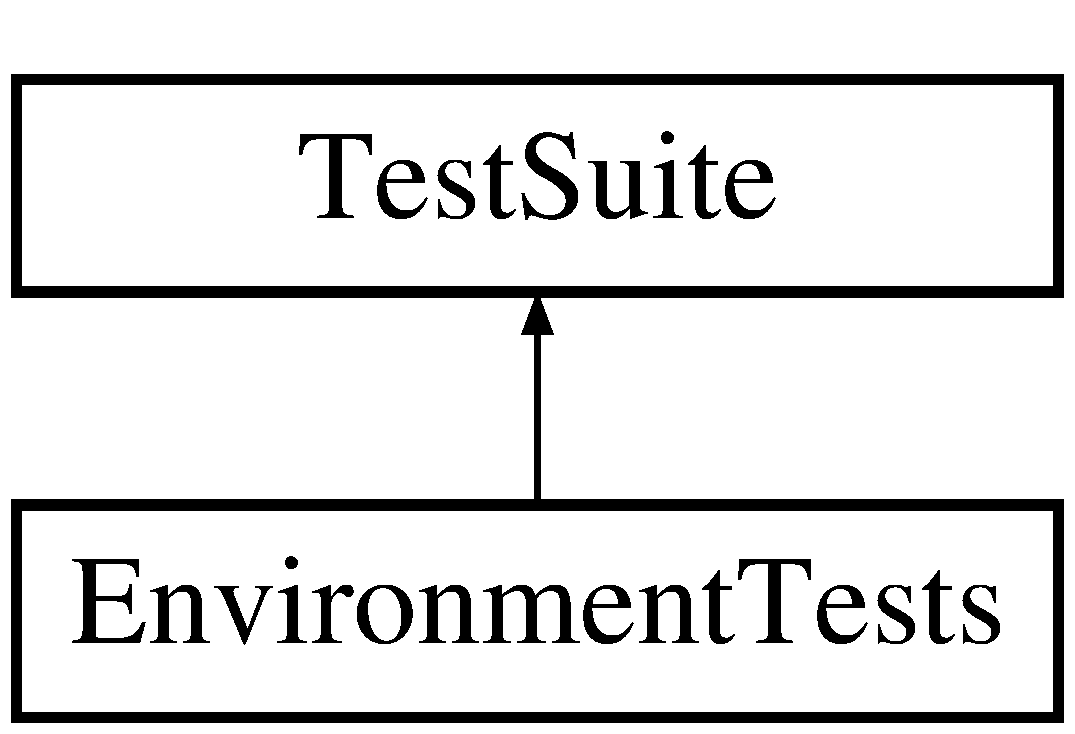
\includegraphics[height=2.000000cm]{classEnvironmentTests}
\end{center}
\end{figure}
\subsection*{Public Member Functions}
\begin{DoxyCompactItemize}
\item 
\hypertarget{classEnvironmentTests_a9899e88cc8aadbce38f3dda949d86cf7}{void {\bfseries test\-Environment\-Properly\-Created} (void)}\label{classEnvironmentTests_a9899e88cc8aadbce38f3dda949d86cf7}

\item 
\hypertarget{classEnvironmentTests_aa467224377550c73dcf88b383bb03c13}{void {\bfseries test\-Get\-Walls} (void)}\label{classEnvironmentTests_aa467224377550c73dcf88b383bb03c13}

\end{DoxyCompactItemize}


The documentation for this class was generated from the following file\-:\begin{DoxyCompactItemize}
\item 
Environment\-Tests.\-hpp\end{DoxyCompactItemize}

\hypertarget{classObstacle}{\section{Obstacle Class Reference}
\label{classObstacle}\index{Obstacle@{Obstacle}}
}


{\ttfamily \#include $<$Obstacle.\-hpp$>$}

Inheritance diagram for Obstacle\-:\begin{figure}[H]
\begin{center}
\leavevmode
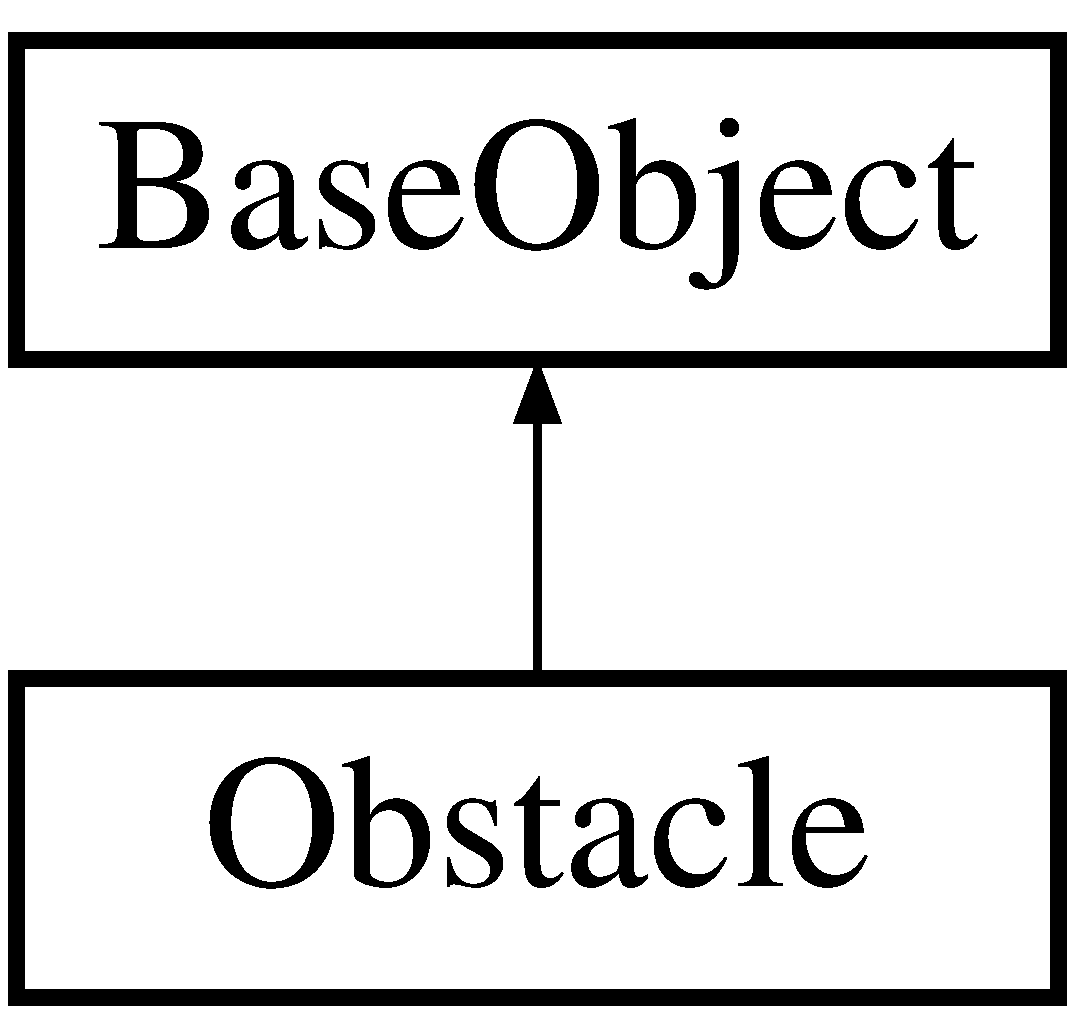
\includegraphics[height=2.000000cm]{classObstacle}
\end{center}
\end{figure}
\subsection*{Public Member Functions}
\begin{DoxyCompactItemize}
\item 
\hyperlink{classObstacle_ad274910c0158000031e8c3e2b1d5d27a}{Obstacle} (int speed\-Rating)
\item 
\hyperlink{classObstacle_af2f9cc9c6cff75dca0974fd5ac4f71a9}{$\sim$\-Obstacle} ()
\item 
std\-::pair$<$ int, int $>$ \hyperlink{classObstacle_aa7ae706f871732fd272bc3d5d066a478}{move} (int elapsed\-Time)
\end{DoxyCompactItemize}
\subsection*{Additional Inherited Members}


\subsection{Detailed Description}
\hyperlink{classObstacle}{Obstacle} Class inherits to Physical Object Class.\-Connect \char`\"{}o\char`\"{} and speed\-Rating. 

\subsection{Constructor \& Destructor Documentation}
\hypertarget{classObstacle_ad274910c0158000031e8c3e2b1d5d27a}{\index{Obstacle@{Obstacle}!Obstacle@{Obstacle}}
\index{Obstacle@{Obstacle}!Obstacle@{Obstacle}}
\subsubsection[{Obstacle}]{\setlength{\rightskip}{0pt plus 5cm}Obstacle\-::\-Obstacle (
\begin{DoxyParamCaption}
\item[{int}]{speed\-Rating}
\end{DoxyParamCaption}
)}}\label{classObstacle_ad274910c0158000031e8c3e2b1d5d27a}
The constructor for the \hyperlink{classObstacle}{Obstacle}

\hyperlink{classObstacle}{Obstacle} Class inherits to Physical Object Class. Connect \char`\"{}o\char`\"{} and speed\-Rating. \hypertarget{classObstacle_af2f9cc9c6cff75dca0974fd5ac4f71a9}{\index{Obstacle@{Obstacle}!$\sim$\-Obstacle@{$\sim$\-Obstacle}}
\index{$\sim$\-Obstacle@{$\sim$\-Obstacle}!Obstacle@{Obstacle}}
\subsubsection[{$\sim$\-Obstacle}]{\setlength{\rightskip}{0pt plus 5cm}Obstacle\-::$\sim$\-Obstacle (
\begin{DoxyParamCaption}
{}
\end{DoxyParamCaption}
)}}\label{classObstacle_af2f9cc9c6cff75dca0974fd5ac4f71a9}
The destructor for the \hyperlink{classObstacle}{Obstacle} class. This frees the \hyperlink{classObstacle}{Obstacle} from memory.

Destructor for the \hyperlink{classObstacle}{Obstacle} 

\subsection{Member Function Documentation}
\hypertarget{classObstacle_aa7ae706f871732fd272bc3d5d066a478}{\index{Obstacle@{Obstacle}!move@{move}}
\index{move@{move}!Obstacle@{Obstacle}}
\subsubsection[{move}]{\setlength{\rightskip}{0pt plus 5cm}std\-::pair$<$ int, int $>$ Obstacle\-::move (
\begin{DoxyParamCaption}
\item[{int}]{elapsed\-Time}
\end{DoxyParamCaption}
)\hspace{0.3cm}{\ttfamily [virtual]}}}\label{classObstacle_aa7ae706f871732fd272bc3d5d066a478}
\hyperlink{classObstacle}{Obstacle} class implement move which will depend on move behavior of a child object. based on elapsed\-Time.

Method which currently \char`\"{}moves\char`\"{} the obstacle by doing nothing. In the future there may be moving objects at which point this method will be more fully implemented Setting the variable of rotate Degree and move\-Forward.

Returen to pair structure. 

Implements \hyperlink{classBaseObject}{Base\-Object}.



The documentation for this class was generated from the following files\-:\begin{DoxyCompactItemize}
\item 
Obstacle.\-hpp\item 
\hyperlink{Obstacle_8cpp}{Obstacle.\-cpp}\end{DoxyCompactItemize}

\hypertarget{classRobot}{\section{Robot Class Reference}
\label{classRobot}\index{Robot@{Robot}}
}


{\ttfamily \#include $<$Robot.\-hpp$>$}

Inheritance diagram for Robot\-:\begin{figure}[H]
\begin{center}
\leavevmode
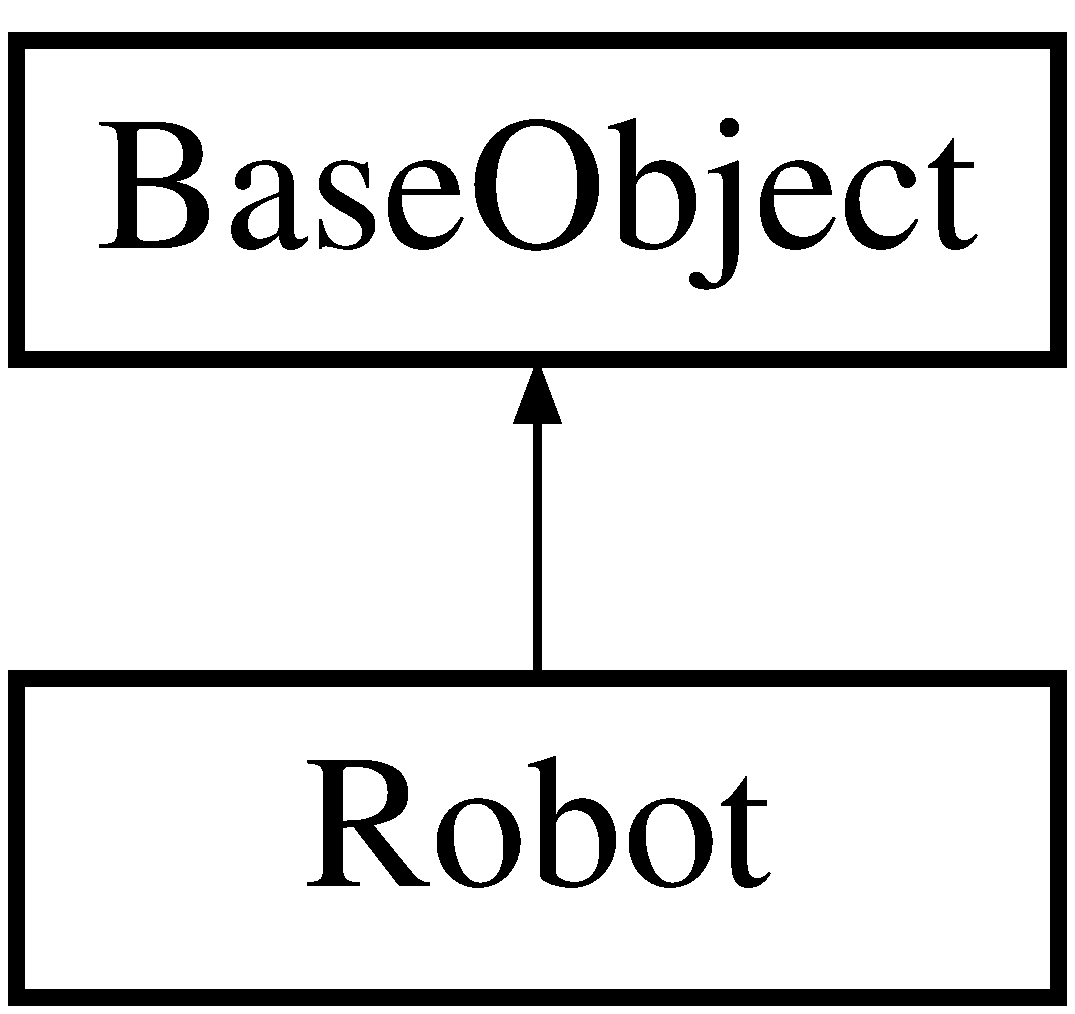
\includegraphics[height=2.000000cm]{classRobot}
\end{center}
\end{figure}
\subsection*{Public Member Functions}
\begin{DoxyCompactItemize}
\item 
\hyperlink{classRobot_afcba47fc04fbe6437521c282b9c5d80f}{Robot} (int speed\-Rating, int size\-Rating)
\item 
\hyperlink{classRobot_a924320124b09c2f2ac1621aa210d5f38}{$\sim$\-Robot} ()
\item 
int \hyperlink{classRobot_a8b7a0c6c281310ae1c4c0df08257599b}{get\-Paired\-Target\-I\-D} ()
\item 
void \hyperlink{classRobot_af594993f7484ac31a480617ac9957fed}{sensor\-Scans} ()
\item 
void \hyperlink{classRobot_ae170cc3e094fd3f82caedb2d7af54824}{pair\-With\-Target} (int target\-I\-D)
\item 
bool \hyperlink{classRobot_af3301a2536ba5bc5aefb7367ccbad6bd}{get\-Collide\-My\-Target} () const 
\item 
std\-::pair$<$ int, int $>$ \hyperlink{classRobot_a4372152d32fc8ccbf51133d9e5f6ad57}{move} (int elapsed\-Time)
\end{DoxyCompactItemize}
\subsection*{Additional Inherited Members}


\subsection{Detailed Description}
\hyperlink{classRobot}{Robot} Class inherits to Physical Object Class.\-Connect \char`\"{}r\char`\"{} and size\-Rating and speed\-Rating. Colliding division. While moving, Collide own and other target(\-Collide\-My\-Target and Collide\-Other\-Target). It must false. 

\subsection{Constructor \& Destructor Documentation}
\hypertarget{classRobot_afcba47fc04fbe6437521c282b9c5d80f}{\index{Robot@{Robot}!Robot@{Robot}}
\index{Robot@{Robot}!Robot@{Robot}}
\subsubsection[{Robot}]{\setlength{\rightskip}{0pt plus 5cm}Robot\-::\-Robot (
\begin{DoxyParamCaption}
\item[{int}]{speed\-Rating, }
\item[{int}]{size\-Rating}
\end{DoxyParamCaption}
)}}\label{classRobot_afcba47fc04fbe6437521c282b9c5d80f}
Constructor which takes as input speed and size ratings which are translated into actual robot radius and speed \hypertarget{classRobot_a924320124b09c2f2ac1621aa210d5f38}{\index{Robot@{Robot}!$\sim$\-Robot@{$\sim$\-Robot}}
\index{$\sim$\-Robot@{$\sim$\-Robot}!Robot@{Robot}}
\subsubsection[{$\sim$\-Robot}]{\setlength{\rightskip}{0pt plus 5cm}Robot\-::$\sim$\-Robot (
\begin{DoxyParamCaption}
{}
\end{DoxyParamCaption}
)}}\label{classRobot_a924320124b09c2f2ac1621aa210d5f38}
Destructor for the \hyperlink{classRobot}{Robot}

Destructor 

\subsection{Member Function Documentation}
\hypertarget{classRobot_af3301a2536ba5bc5aefb7367ccbad6bd}{\index{Robot@{Robot}!get\-Collide\-My\-Target@{get\-Collide\-My\-Target}}
\index{get\-Collide\-My\-Target@{get\-Collide\-My\-Target}!Robot@{Robot}}
\subsubsection[{get\-Collide\-My\-Target}]{\setlength{\rightskip}{0pt plus 5cm}bool Robot\-::get\-Collide\-My\-Target (
\begin{DoxyParamCaption}
{}
\end{DoxyParamCaption}
) const}}\label{classRobot_af3301a2536ba5bc5aefb7367ccbad6bd}
Colliding with own target

Method returns true if the object is colliding with its own target \hypertarget{classRobot_a8b7a0c6c281310ae1c4c0df08257599b}{\index{Robot@{Robot}!get\-Paired\-Target\-I\-D@{get\-Paired\-Target\-I\-D}}
\index{get\-Paired\-Target\-I\-D@{get\-Paired\-Target\-I\-D}!Robot@{Robot}}
\subsubsection[{get\-Paired\-Target\-I\-D}]{\setlength{\rightskip}{0pt plus 5cm}int Robot\-::get\-Paired\-Target\-I\-D (
\begin{DoxyParamCaption}
{}
\end{DoxyParamCaption}
)}}\label{classRobot_a8b7a0c6c281310ae1c4c0df08257599b}
Checking to Target\-I\-D

Method which returns the I\-D of the paired target \hypertarget{classRobot_a4372152d32fc8ccbf51133d9e5f6ad57}{\index{Robot@{Robot}!move@{move}}
\index{move@{move}!Robot@{Robot}}
\subsubsection[{move}]{\setlength{\rightskip}{0pt plus 5cm}std\-::pair$<$ int, int $>$ Robot\-::move (
\begin{DoxyParamCaption}
\item[{int}]{elapsed\-Time}
\end{DoxyParamCaption}
)\hspace{0.3cm}{\ttfamily [virtual]}}}\label{classRobot_a4372152d32fc8ccbf51133d9e5f6ad57}
\hyperlink{classRobot}{Robot} class implement move which will depend on move behavior of a child object. based on elapsed\-Time. Calculate elapsed\-Time divide 1000 and multiply speed. This means move\-Forward. When we collide obstacle, target, robot,or wall, we change the degree 91. \hyperlink{classRobot}{Robot} class has a target signal for knowing which target hit.

Method which determines the proper movement of the object based on the elapsed time 

Implements \hyperlink{classBaseObject}{Base\-Object}.

\hypertarget{classRobot_ae170cc3e094fd3f82caedb2d7af54824}{\index{Robot@{Robot}!pair\-With\-Target@{pair\-With\-Target}}
\index{pair\-With\-Target@{pair\-With\-Target}!Robot@{Robot}}
\subsubsection[{pair\-With\-Target}]{\setlength{\rightskip}{0pt plus 5cm}void Robot\-::pair\-With\-Target (
\begin{DoxyParamCaption}
\item[{int}]{target\-I\-D}
\end{DoxyParamCaption}
)}}\label{classRobot_ae170cc3e094fd3f82caedb2d7af54824}
Calling pair \hyperlink{classTarget}{Target} information.

Method which sets the member variable holding the robot's paired target I\-D \hypertarget{classRobot_af594993f7484ac31a480617ac9957fed}{\index{Robot@{Robot}!sensor\-Scans@{sensor\-Scans}}
\index{sensor\-Scans@{sensor\-Scans}!Robot@{Robot}}
\subsubsection[{sensor\-Scans}]{\setlength{\rightskip}{0pt plus 5cm}void Robot\-::sensor\-Scans (
\begin{DoxyParamCaption}
{}
\end{DoxyParamCaption}
)\hspace{0.3cm}{\ttfamily [virtual]}}}\label{classRobot_af594993f7484ac31a480617ac9957fed}
\hyperlink{classRobot}{Robot} sensor\-Scan have touchsensor and homingsensor. According to id, \hyperlink{classRobot}{Robot} determine moving.

Method which scans environment, collecting touch and homing readings. Also analyzes collisions looking for a collision with its own target 

Reimplemented from \hyperlink{classBaseObject}{Base\-Object}.



The documentation for this class was generated from the following files\-:\begin{DoxyCompactItemize}
\item 
\hyperlink{Robot_8hpp}{Robot.\-hpp}\item 
\hyperlink{Robot_8cpp}{Robot.\-cpp}\end{DoxyCompactItemize}

\hypertarget{classRobotTests}{\section{Robot\-Tests Class Reference}
\label{classRobotTests}\index{Robot\-Tests@{Robot\-Tests}}
}
Inheritance diagram for Robot\-Tests\-:\begin{figure}[H]
\begin{center}
\leavevmode
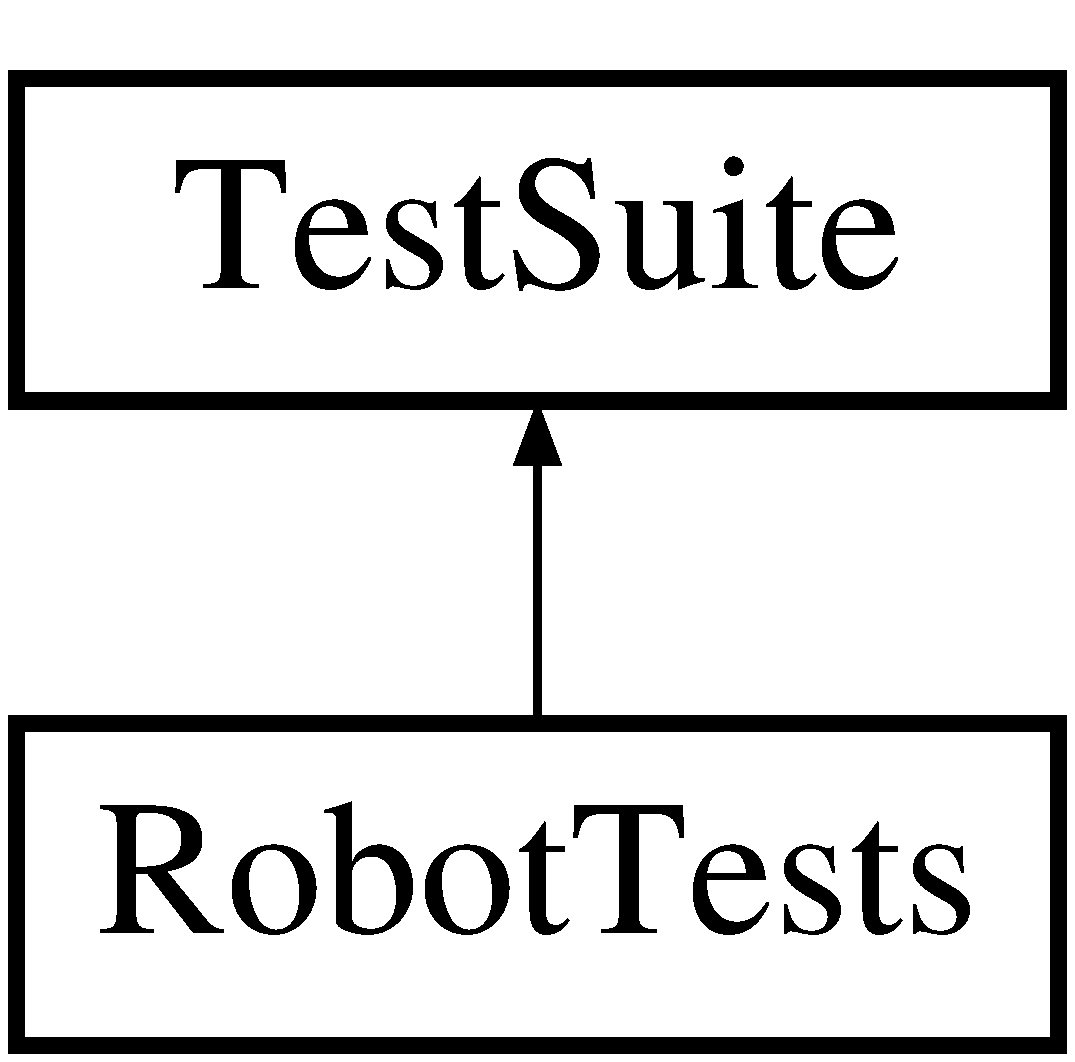
\includegraphics[height=2.000000cm]{classRobotTests}
\end{center}
\end{figure}
\subsection*{Public Member Functions}
\begin{DoxyCompactItemize}
\item 
\hypertarget{classRobotTests_a13488190dfd219240f08d0ec9409ff83}{void {\bfseries test\-Get\-Paired\-Target} (void)}\label{classRobotTests_a13488190dfd219240f08d0ec9409ff83}

\item 
\hypertarget{classRobotTests_a253d41ed299372c25bfef3e805cfa94f}{void {\bfseries test\-Sensor\-Scans} (void)}\label{classRobotTests_a253d41ed299372c25bfef3e805cfa94f}

\item 
\hypertarget{classRobotTests_aaa7edcf5849e5005e4b7ca247b3b2668}{void {\bfseries test\-Pair\-With\-Target} (void)}\label{classRobotTests_aaa7edcf5849e5005e4b7ca247b3b2668}

\item 
\hypertarget{classRobotTests_a9e3ef94640baa0034c0ee73b188b917f}{void {\bfseries test\-Get\-Collide\-My\-Target} (void)}\label{classRobotTests_a9e3ef94640baa0034c0ee73b188b917f}

\item 
\hypertarget{classRobotTests_a4d331c44ef8b4b5fe1d70207f68ff1ab}{void {\bfseries test\-Move} (void)}\label{classRobotTests_a4d331c44ef8b4b5fe1d70207f68ff1ab}

\end{DoxyCompactItemize}


The documentation for this class was generated from the following file\-:\begin{DoxyCompactItemize}
\item 
Robot\-Tests.\-hpp\end{DoxyCompactItemize}

\hypertarget{classSimulation}{\section{Simulation Class Reference}
\label{classSimulation}\index{Simulation@{Simulation}}
}


{\ttfamily \#include $<$Simulation.\-hpp$>$}

Inheritance diagram for Simulation\-:\begin{figure}[H]
\begin{center}
\leavevmode
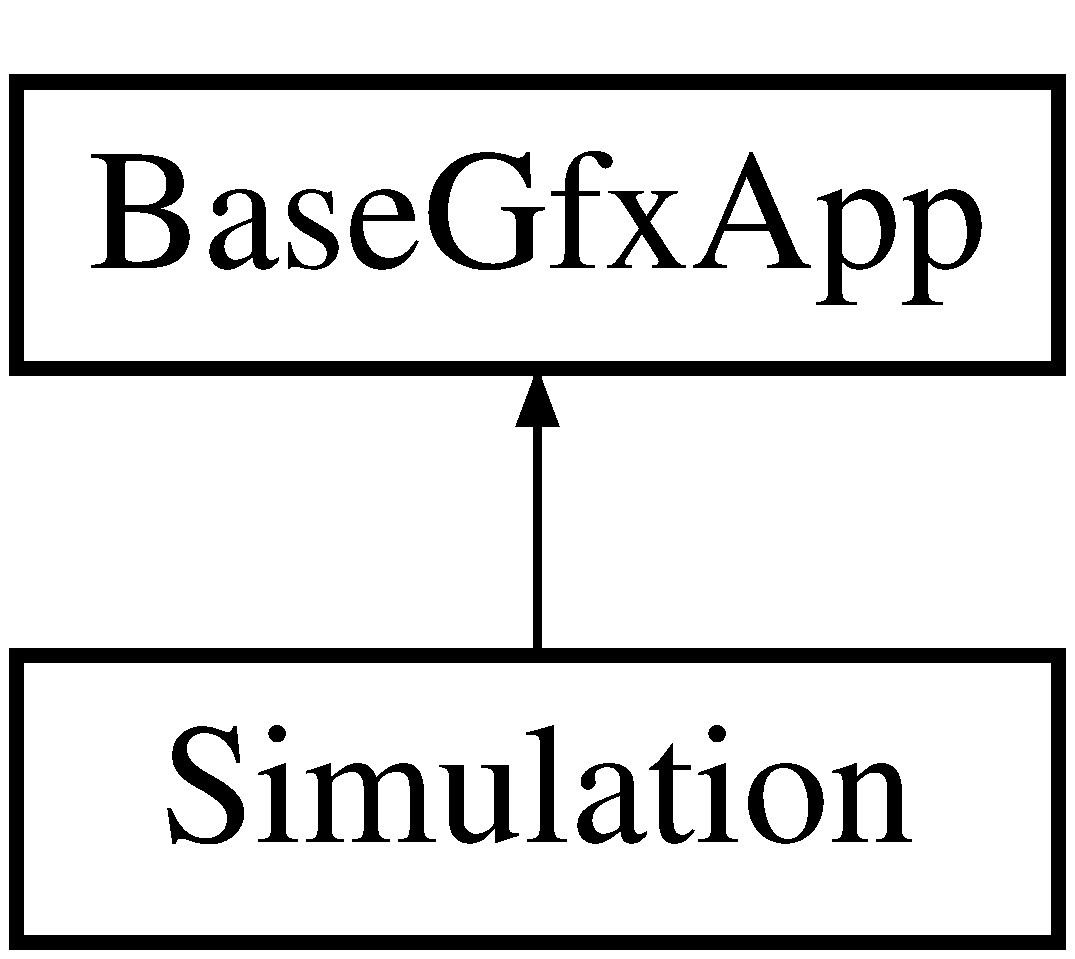
\includegraphics[height=2.000000cm]{classSimulation}
\end{center}
\end{figure}
\subsection*{Public Types}
\begin{DoxyCompactItemize}
\item 
enum {\bfseries U\-I\-Control\-Type} \{ {\bfseries U\-I\-\_\-\-Q\-U\-I\-T} = 0, 
{\bfseries U\-I\-\_\-\-S\-T\-A\-R\-T} = 1, 
{\bfseries U\-I\-\_\-\-P\-A\-U\-S\-E} = 2, 
{\bfseries U\-I\-\_\-\-R\-E\-S\-U\-M\-E} = 3
 \}
\end{DoxyCompactItemize}
\subsection*{Public Member Functions}
\begin{DoxyCompactItemize}
\item 
\hyperlink{classSimulation_a4c669ceaa34c7130966ce45f9de75fbe}{Simulation} (int argc, char $\ast$argv\mbox{[}$\,$\mbox{]}, int width, int height)
\item 
void \hyperlink{classSimulation_a449dcb7d97dfba99efe770de2f399c31}{display} ()
\item 
\hypertarget{classSimulation_a1607cd18e552ab9f4a6f57d362f7121a}{void {\bfseries glui\-Control} (int control\-I\-D)}\label{classSimulation_a1607cd18e552ab9f4a6f57d362f7121a}

\item 
\hypertarget{classSimulation_a786d1ba31d29937f0ac6f3ea88f8a607}{void {\bfseries left\-Mouse\-Down} (int x, int y)}\label{classSimulation_a786d1ba31d29937f0ac6f3ea88f8a607}

\item 
\hypertarget{classSimulation_a62ef254d85017074cd521a5787b5a234}{void {\bfseries left\-Mouse\-Up} (int x, int y)}\label{classSimulation_a62ef254d85017074cd521a5787b5a234}

\end{DoxyCompactItemize}
\subsection*{Additional Inherited Members}


\subsection{Detailed Description}
The \hyperlink{classSimulation}{Simulation} class. This sets up the G\-U\-I and the drawing environment. 

\subsection{Constructor \& Destructor Documentation}
\hypertarget{classSimulation_a4c669ceaa34c7130966ce45f9de75fbe}{\index{Simulation@{Simulation}!Simulation@{Simulation}}
\index{Simulation@{Simulation}!Simulation@{Simulation}}
\subsubsection[{Simulation}]{\setlength{\rightskip}{0pt plus 5cm}Simulation\-::\-Simulation (
\begin{DoxyParamCaption}
\item[{int}]{argc, }
\item[{char $\ast$}]{argv\mbox{[}$\,$\mbox{]}, }
\item[{int}]{width, }
\item[{int}]{height}
\end{DoxyParamCaption}
)}}\label{classSimulation_a4c669ceaa34c7130966ce45f9de75fbe}
The constructor for the \hyperlink{classSimulation}{Simulation} class. It does all setup for the display. In particular, the initial values are set for the robot, obstacles, target, and walls. It takes four parameters\-: the number of console arguments, their values, and the width and height of the screen in pixels. 
\begin{DoxyParams}{Parameters}
{\em argc} & The number of arguments supplied on the command line. \\
\hline
{\em argv\mbox{[}$\,$\mbox{]}} & The values of the arguments supplied on the command line. \\
\hline
{\em width} & The width of the screen measured in pixels. \\
\hline
{\em height} & The height of the screen measured in pixels. \\
\hline
\end{DoxyParams}
Creating the environment 

\subsection{Member Function Documentation}
\hypertarget{classSimulation_a449dcb7d97dfba99efe770de2f399c31}{\index{Simulation@{Simulation}!display@{display}}
\index{display@{display}!Simulation@{Simulation}}
\subsubsection[{display}]{\setlength{\rightskip}{0pt plus 5cm}void Simulation\-::display (
\begin{DoxyParamCaption}
{}
\end{DoxyParamCaption}
)\hspace{0.3cm}{\ttfamily [virtual]}}}\label{classSimulation_a449dcb7d97dfba99efe770de2f399c31}
This public method coordinates the display at every screen refresh. It calls the private methods which perform the actual work of drawing agents, indicators, and walls to the screen. Updating the time counters keeping track of total time since the simulation began as well as the elapsed time since the last update.

Updating the true environment based on the time since the last update

Updating the environment as depicted in the simulation screen 

Reimplemented from \hyperlink{classBaseGfxApp}{Base\-Gfx\-App}.



The documentation for this class was generated from the following files\-:\begin{DoxyCompactItemize}
\item 
\hyperlink{Simulation_8hpp}{Simulation.\-hpp}\item 
\hyperlink{Simulation_8cpp}{Simulation.\-cpp}\end{DoxyCompactItemize}

\hypertarget{classTarget}{\section{Target Class Reference}
\label{classTarget}\index{Target@{Target}}
}


{\ttfamily \#include $<$Target.\-hpp$>$}

Inheritance diagram for Target\-:\begin{figure}[H]
\begin{center}
\leavevmode
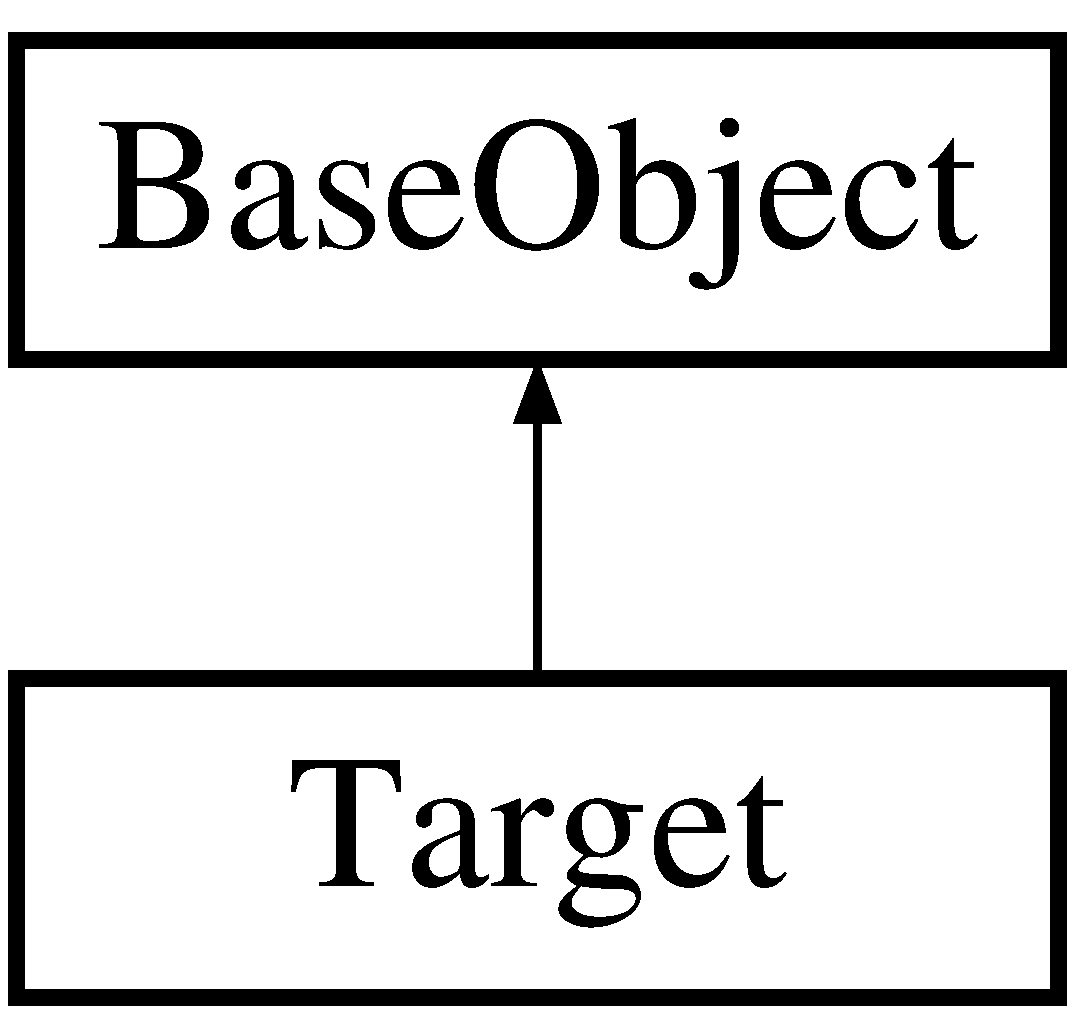
\includegraphics[height=2.000000cm]{classTarget}
\end{center}
\end{figure}
\subsection*{Public Member Functions}
\begin{DoxyCompactItemize}
\item 
\hyperlink{classTarget_a343a7c2b7aa4eb1437c1202a0588e87b}{Target} (int speed\-Rating, int size\-Rating)
\item 
\hyperlink{classTarget_a18102a6c58a268fb1466771463fdc9b3}{$\sim$\-Target} ()
\item 
std\-::pair$<$ int, int $>$ \hyperlink{classTarget_a5a664acae049600db8f53e25f613ac81}{move} (int elapsed\-Time)
\item 
void \hyperlink{classTarget_a0d5f00e2e5587dfc2a4ee89a8bf91b35}{sensor\-Scans} ()
\end{DoxyCompactItemize}
\subsection*{Additional Inherited Members}


\subsection{Detailed Description}
\hyperlink{classTarget}{Target} Class inherits to Physical Object Class.\-Connect \char`\"{}t\char`\"{} and size\-Rating. 

\subsection{Constructor \& Destructor Documentation}
\hypertarget{classTarget_a343a7c2b7aa4eb1437c1202a0588e87b}{\index{Target@{Target}!Target@{Target}}
\index{Target@{Target}!Target@{Target}}
\subsubsection[{Target}]{\setlength{\rightskip}{0pt plus 5cm}Target\-::\-Target (
\begin{DoxyParamCaption}
\item[{int}]{speed\-Rating, }
\item[{int}]{size\-Rating}
\end{DoxyParamCaption}
)}}\label{classTarget_a343a7c2b7aa4eb1437c1202a0588e87b}
The constructor for the \hyperlink{classTarget}{Target}

Constructor. Takes as input a speed rating between 0-\/100 and size rating between 1-\/100. The object's actual speed and radius are set accordingly \hypertarget{classTarget_a18102a6c58a268fb1466771463fdc9b3}{\index{Target@{Target}!$\sim$\-Target@{$\sim$\-Target}}
\index{$\sim$\-Target@{$\sim$\-Target}!Target@{Target}}
\subsubsection[{$\sim$\-Target}]{\setlength{\rightskip}{0pt plus 5cm}Target\-::$\sim$\-Target (
\begin{DoxyParamCaption}
{}
\end{DoxyParamCaption}
)}}\label{classTarget_a18102a6c58a268fb1466771463fdc9b3}
The destructor for the \hyperlink{classTarget}{Target} class. This frees the \hyperlink{classTarget}{Target} from memory.

Destructor for the \hyperlink{classTarget}{Target} 

\subsection{Member Function Documentation}
\hypertarget{classTarget_a5a664acae049600db8f53e25f613ac81}{\index{Target@{Target}!move@{move}}
\index{move@{move}!Target@{Target}}
\subsubsection[{move}]{\setlength{\rightskip}{0pt plus 5cm}std\-::pair$<$ int, int $>$ Target\-::move (
\begin{DoxyParamCaption}
\item[{int}]{elapsed\-Time}
\end{DoxyParamCaption}
)\hspace{0.3cm}{\ttfamily [virtual]}}}\label{classTarget_a5a664acae049600db8f53e25f613ac81}
Targetclass implement move which will depend on move behavior of a child object. based on elapsed\-Time. Calculate elapsed\-Time divide 1000 and multiply speed. This means move\-Forward. When we collide obstacle, target, robot,or wall, we change the degree 91.

Method which determines target movement decisions based on the elapsed time and whether or not the target is colliding with other objects 

Implements \hyperlink{classBaseObject}{Base\-Object}.

\hypertarget{classTarget_a0d5f00e2e5587dfc2a4ee89a8bf91b35}{\index{Target@{Target}!sensor\-Scans@{sensor\-Scans}}
\index{sensor\-Scans@{sensor\-Scans}!Target@{Target}}
\subsubsection[{sensor\-Scans}]{\setlength{\rightskip}{0pt plus 5cm}void Target\-::sensor\-Scans (
\begin{DoxyParamCaption}
{}
\end{DoxyParamCaption}
)\hspace{0.3cm}{\ttfamily [virtual]}}}\label{classTarget_a0d5f00e2e5587dfc2a4ee89a8bf91b35}
Targetclass provide current position based on sensory feedback including id and pair vector.

Targetclass provides current position based on sensory feedback including id and pair vector. 

Reimplemented from \hyperlink{classBaseObject}{Base\-Object}.



The documentation for this class was generated from the following files\-:\begin{DoxyCompactItemize}
\item 
\hyperlink{Target_8hpp}{Target.\-hpp}\item 
\hyperlink{Target_8cpp}{Target.\-cpp}\end{DoxyCompactItemize}

\hypertarget{classWalls}{\section{Walls Class Reference}
\label{classWalls}\index{Walls@{Walls}}
}


{\ttfamily \#include $<$Walls.\-hpp$>$}

\subsection*{Public Member Functions}
\begin{DoxyCompactItemize}
\item 
\hyperlink{classWalls_a8c5996222aa9dad4af6528d88110fd28}{Walls} (int app\-Width, int app\-Height)
\item 
\hyperlink{classWalls_a1136e53ddf2cc39aa354e9a02ec98f43}{$\sim$\-Walls} ()
\item 
int \hyperlink{classWalls_a360fb70538bfd72d05ba9b011ac4f7bb}{get\-Width} () const 
\item 
int \hyperlink{classWalls_a696765c4b969fbe387d03d7c469c6e16}{get\-Height} () const 
\item 
int \hyperlink{classWalls_a7b781a5d6151546dfcdde4981f44f0c9}{get\-Thickness} () const 
\end{DoxyCompactItemize}


\subsection{Detailed Description}
\hyperlink{classWalls}{Walls} class, which is used to form a collision boundary around the perimeter of the window 

\subsection{Constructor \& Destructor Documentation}
\hypertarget{classWalls_a8c5996222aa9dad4af6528d88110fd28}{\index{Walls@{Walls}!Walls@{Walls}}
\index{Walls@{Walls}!Walls@{Walls}}
\subsubsection[{Walls}]{\setlength{\rightskip}{0pt plus 5cm}Walls\-::\-Walls (
\begin{DoxyParamCaption}
\item[{int}]{app\-Width, }
\item[{int}]{app\-Height}
\end{DoxyParamCaption}
)}}\label{classWalls_a8c5996222aa9dad4af6528d88110fd28}
The constructor for the \hyperlink{classWalls}{Walls} class takes two parameters\-: app\-Height and app\-Width. 
\begin{DoxyParams}{Parameters}
{\em app\-Height} & The height of the \hyperlink{classWalls}{Walls} of the window in pixels. \\
\hline
{\em app\-Width} & The width of the \hyperlink{classWalls}{Walls} of the window in pixels. \\
\hline
\end{DoxyParams}
\hypertarget{classWalls_a1136e53ddf2cc39aa354e9a02ec98f43}{\index{Walls@{Walls}!$\sim$\-Walls@{$\sim$\-Walls}}
\index{$\sim$\-Walls@{$\sim$\-Walls}!Walls@{Walls}}
\subsubsection[{$\sim$\-Walls}]{\setlength{\rightskip}{0pt plus 5cm}Walls\-::$\sim$\-Walls (
\begin{DoxyParamCaption}
{}
\end{DoxyParamCaption}
)}}\label{classWalls_a1136e53ddf2cc39aa354e9a02ec98f43}
Wall destructor. 

\subsection{Member Function Documentation}
\hypertarget{classWalls_a696765c4b969fbe387d03d7c469c6e16}{\index{Walls@{Walls}!get\-Height@{get\-Height}}
\index{get\-Height@{get\-Height}!Walls@{Walls}}
\subsubsection[{get\-Height}]{\setlength{\rightskip}{0pt plus 5cm}int Walls\-::get\-Height (
\begin{DoxyParamCaption}
{}
\end{DoxyParamCaption}
) const}}\label{classWalls_a696765c4b969fbe387d03d7c469c6e16}
Returns the height of the wall in pixels. \hypertarget{classWalls_a7b781a5d6151546dfcdde4981f44f0c9}{\index{Walls@{Walls}!get\-Thickness@{get\-Thickness}}
\index{get\-Thickness@{get\-Thickness}!Walls@{Walls}}
\subsubsection[{get\-Thickness}]{\setlength{\rightskip}{0pt plus 5cm}int Walls\-::get\-Thickness (
\begin{DoxyParamCaption}
{}
\end{DoxyParamCaption}
) const}}\label{classWalls_a7b781a5d6151546dfcdde4981f44f0c9}
Returns the thickness of the wall in pixels. \hypertarget{classWalls_a360fb70538bfd72d05ba9b011ac4f7bb}{\index{Walls@{Walls}!get\-Width@{get\-Width}}
\index{get\-Width@{get\-Width}!Walls@{Walls}}
\subsubsection[{get\-Width}]{\setlength{\rightskip}{0pt plus 5cm}int Walls\-::get\-Width (
\begin{DoxyParamCaption}
{}
\end{DoxyParamCaption}
) const}}\label{classWalls_a360fb70538bfd72d05ba9b011ac4f7bb}
Returns the width of the wall in pixels. 

The documentation for this class was generated from the following files\-:\begin{DoxyCompactItemize}
\item 
\hyperlink{Walls_8hpp}{Walls.\-hpp}\item 
\hyperlink{Walls_8cpp}{Walls.\-cpp}\end{DoxyCompactItemize}

\chapter{File Documentation}
\hypertarget{BaseGfxApp_8hpp}{\section{Base\-Gfx\-App.\-hpp File Reference}
\label{BaseGfxApp_8hpp}\index{Base\-Gfx\-App.\-hpp@{Base\-Gfx\-App.\-hpp}}
}


The basic application class for C\-Sci-\/3081 project. Uses G\-L\-U\-T and G\-L\-U\-I and wraps them in a nice C++ interface.  


{\ttfamily \#include $<$string$>$}\\*
{\ttfamily \#include $<$iostream$>$}\\*
{\ttfamily \#include $<$assert.\-h$>$}\\*
{\ttfamily \#include \char`\"{}../lib/glui/include/\-G\-L/glui.\-h\char`\"{}}\\*
\subsection*{Classes}
\begin{DoxyCompactItemize}
\item 
class \hyperlink{classBaseGfxApp}{Base\-Gfx\-App}
\end{DoxyCompactItemize}


\subsection{Detailed Description}
The basic application class for C\-Sci-\/3081 project. Uses G\-L\-U\-T and G\-L\-U\-I and wraps them in a nice C++ interface. \begin{DoxyAuthor}{Author}
C\-Sci3081 Starter Code 
\end{DoxyAuthor}

\hypertarget{BaseObject_8hpp}{\section{Base\-Object.\-hpp File Reference}
\label{BaseObject_8hpp}\index{Base\-Object.\-hpp@{Base\-Object.\-hpp}}
}


The base class which all other physical objects derive from. It contains core data relevant to all objects, such as speed, size, color, object id number, and collision logic.  


{\ttfamily \#include $<$utility$>$}\\*
{\ttfamily \#include $<$tuple$>$}\\*
{\ttfamily \#include \char`\"{}Environment.\-hpp\char`\"{}}\\*
\subsection*{Classes}
\begin{DoxyCompactItemize}
\item 
class \hyperlink{classBaseObject}{Base\-Object}
\end{DoxyCompactItemize}


\subsection{Detailed Description}
The base class which all other physical objects derive from. It contains core data relevant to all objects, such as speed, size, color, object id number, and collision logic. \begin{DoxyAuthor}{Author}
George Brown 
\end{DoxyAuthor}

\hypertarget{Environment_8hpp}{\section{Environment.\-hpp File Reference}
\label{Environment_8hpp}\index{Environment.\-hpp@{Environment.\-hpp}}
}


The declaration for the enviromnet class. This class explain to update and touch sensor and homing sensor. This class serves as a parent for Physical object Class, The physical object class include collisionstatus, object color, radius, and orientaion.  


{\ttfamily \#include $<$vector$>$}\\*
{\ttfamily \#include $<$utility$>$}\\*
{\ttfamily \#include \char`\"{}Base\-Object.\-hpp\char`\"{}}\\*
{\ttfamily \#include \char`\"{}Walls.\-hpp\char`\"{}}\\*
\subsection*{Classes}
\begin{DoxyCompactItemize}
\item 
class \hyperlink{classEnvironment}{Environment}
\end{DoxyCompactItemize}


\subsection{Detailed Description}
The declaration for the enviromnet class. This class explain to update and touch sensor and homing sensor. This class serves as a parent for Physical object Class, The physical object class include collisionstatus, object color, radius, and orientaion. \begin{DoxyAuthor}{Author}
George Brown 
\end{DoxyAuthor}

\hypertarget{main_8cpp}{\section{main.\-cpp File Reference}
\label{main_8cpp}\index{main.\-cpp@{main.\-cpp}}
}


Main function.  


{\ttfamily \#include \char`\"{}Simulation.\-hpp\char`\"{}}\\*
{\ttfamily \#include $<$ctime$>$}\\*
\subsection*{Functions}
\begin{DoxyCompactItemize}
\item 
\hypertarget{main_8cpp_a0ddf1224851353fc92bfbff6f499fa97}{int {\bfseries main} (int argc, char $\ast$argv\mbox{[}$\,$\mbox{]})}\label{main_8cpp_a0ddf1224851353fc92bfbff6f499fa97}

\end{DoxyCompactItemize}


\subsection{Detailed Description}
Main function. \begin{DoxyAuthor}{Author}
C\-Sci5107 Guru 
\end{DoxyAuthor}

\hypertarget{Obstacle_8cpp}{\section{Obstacle.\-cpp File Reference}
\label{Obstacle_8cpp}\index{Obstacle.\-cpp@{Obstacle.\-cpp}}
}


Class definition for the \hyperlink{classObstacle}{Obstacle} (child class of \hyperlink{classEnvironment}{Environment}). An obstacle inherits all of its methods from its parent. Improving the code, obstacles have their own unique methods and data. \hyperlink{classEnvironment}{Environment} Class \hyperlink{classEnvironment}{Environment} with static data structure that hold obstacle objects.\-Iteration through the object and moving them based on elasped\-Time.  


{\ttfamily \#include \char`\"{}Obstacle.\-hpp\char`\"{}}\\*


\subsection{Detailed Description}
Class definition for the \hyperlink{classObstacle}{Obstacle} (child class of \hyperlink{classEnvironment}{Environment}). An obstacle inherits all of its methods from its parent. Improving the code, obstacles have their own unique methods and data. \hyperlink{classEnvironment}{Environment} Class \hyperlink{classEnvironment}{Environment} with static data structure that hold obstacle objects.\-Iteration through the object and moving them based on elasped\-Time. \begin{DoxyAuthor}{Author}
George Brown 
\end{DoxyAuthor}

\hypertarget{Robot_8cpp}{\section{Robot.\-cpp File Reference}
\label{Robot_8cpp}\index{Robot.\-cpp@{Robot.\-cpp}}
}


A robot inherits much of its methods from its parent. However, it also extends it by adding robot-\/specific methods such as point\-To, which points the robot at a target. Future functionality will have the robot controlled by the user physically pressing keys, which will be distinct from how other agents are manipulated.  


{\ttfamily \#include \char`\"{}Robot.\-hpp\char`\"{}}\\*
{\ttfamily \#include $<$iostream$>$}\\*
\subsection*{Typedefs}
\begin{DoxyCompactItemize}
\item 
typedef std\-::vector$<$ std\-::pair\\*
$<$ int, char $>$ $>$ \hyperlink{Robot_8cpp_a7f22ec3bcddc803dd2a219a2beb12ded}{Collide\-Vector\-Pair}
\end{DoxyCompactItemize}


\subsection{Detailed Description}
A robot inherits much of its methods from its parent. However, it also extends it by adding robot-\/specific methods such as point\-To, which points the robot at a target. Future functionality will have the robot controlled by the user physically pressing keys, which will be distinct from how other agents are manipulated. \begin{DoxyAuthor}{Author}
George Brown 
\end{DoxyAuthor}


\subsection{Typedef Documentation}
\hypertarget{Robot_8cpp_a7f22ec3bcddc803dd2a219a2beb12ded}{\index{Robot.\-cpp@{Robot.\-cpp}!Collide\-Vector\-Pair@{Collide\-Vector\-Pair}}
\index{Collide\-Vector\-Pair@{Collide\-Vector\-Pair}!Robot.cpp@{Robot.\-cpp}}
\subsubsection[{Collide\-Vector\-Pair}]{\setlength{\rightskip}{0pt plus 5cm}typedef std\-::vector$<$ std\-::pair$<$int,char$>$ $>$ Collide\-Vector\-Pair}}\label{Robot_8cpp_a7f22ec3bcddc803dd2a219a2beb12ded}
Method analyzes the target collisions to see whether it is colliding with its own target, some other target, both, or neither 
\hypertarget{Robot_8hpp}{\section{Robot.\-hpp File Reference}
\label{Robot_8hpp}\index{Robot.\-hpp@{Robot.\-hpp}}
}


Class definition for the \hyperlink{classRobot}{Robot} (child class of \hyperlink{classEnvironment}{Environment}). A robot inherits much of its methods from its parent. However, it also extends it by adding robot-\/specific methods such as point\-To, which points the robot at a target. Improving the iteration 2 code, \hyperlink{classRobot}{Robot} adding to sensor about touch and homing. Being able to collide obstacle, \hyperlink{classRobot}{Robot} adding to recognize the target and obstacle.  


{\ttfamily \#include \char`\"{}Base\-Object.\-hpp\char`\"{}}\\*
{\ttfamily \#include \char`\"{}Robot.\-hpp\char`\"{}}\\*
\subsection*{Classes}
\begin{DoxyCompactItemize}
\item 
class \hyperlink{classRobot}{Robot}
\end{DoxyCompactItemize}


\subsection{Detailed Description}
Class definition for the \hyperlink{classRobot}{Robot} (child class of \hyperlink{classEnvironment}{Environment}). A robot inherits much of its methods from its parent. However, it also extends it by adding robot-\/specific methods such as point\-To, which points the robot at a target. Improving the iteration 2 code, \hyperlink{classRobot}{Robot} adding to sensor about touch and homing. Being able to collide obstacle, \hyperlink{classRobot}{Robot} adding to recognize the target and obstacle. \begin{DoxyAuthor}{Author}
George Brown 
\end{DoxyAuthor}

\hypertarget{Simulation_8cpp}{\section{Simulation.\-cpp File Reference}
\label{Simulation_8cpp}\index{Simulation.\-cpp@{Simulation.\-cpp}}
}


Main application class for the robot simulation.  


{\ttfamily \#include \char`\"{}Simulation.\-hpp\char`\"{}}\\*
{\ttfamily \#include $<$iostream$>$}\\*
\subsection*{Macros}
\begin{DoxyCompactItemize}
\item 
\hypertarget{Simulation_8cpp_a598a3330b3c21701223ee0ca14316eca}{\#define {\bfseries P\-I}~3.\-1415926535f}\label{Simulation_8cpp_a598a3330b3c21701223ee0ca14316eca}

\end{DoxyCompactItemize}


\subsection{Detailed Description}
Main application class for the robot simulation. \begin{DoxyAuthor}{Author}
C\-Sci3081 Guru 
\end{DoxyAuthor}

\hypertarget{Simulation_8hpp}{\section{Simulation.\-hpp File Reference}
\label{Simulation_8hpp}\index{Simulation.\-hpp@{Simulation.\-hpp}}
}


Main application class for the robot simulation.  


{\ttfamily \#include $<$vector$>$}\\*
{\ttfamily \#include $<$tuple$>$}\\*
{\ttfamily \#include $<$cmath$>$}\\*
{\ttfamily \#include \char`\"{}Walls.\-hpp\char`\"{}}\\*
{\ttfamily \#include \char`\"{}Base\-Gfx\-App.\-hpp\char`\"{}}\\*
{\ttfamily \#include \char`\"{}Robot.\-hpp\char`\"{}}\\*
{\ttfamily \#include \char`\"{}Obstacle.\-hpp\char`\"{}}\\*
\subsection*{Classes}
\begin{DoxyCompactItemize}
\item 
class \hyperlink{classSimulation}{Simulation}
\end{DoxyCompactItemize}


\subsection{Detailed Description}
Main application class for the robot simulation. \begin{DoxyAuthor}{Author}
C\-Sci3081 Guru 
\end{DoxyAuthor}

\hypertarget{Target_8cpp}{\section{Target.\-cpp File Reference}
\label{Target_8cpp}\index{Target.\-cpp@{Target.\-cpp}}
}


Objects of this type will be targets that the robot points to. A target inherits all of its methods from its parent. However, in the future targets may have their own unique methods and data.  


{\ttfamily \#include \char`\"{}Target.\-hpp\char`\"{}}\\*


\subsection{Detailed Description}
Objects of this type will be targets that the robot points to. A target inherits all of its methods from its parent. However, in the future targets may have their own unique methods and data. \begin{DoxyAuthor}{Author}
George Brown, Duk\-Jin Ahn 
\end{DoxyAuthor}

\hypertarget{Target_8hpp}{\section{Target.\-hpp File Reference}
\label{Target_8hpp}\index{Target.\-hpp@{Target.\-hpp}}
}


Class definition for the \hyperlink{classTarget}{Target} (child class of \hyperlink{classEnvironment}{Environment}). An Objects of this type will be targets that the robot points to. A target inherits all of its methods from its parent. Improving the code, targets may have their own unique methods and data. \hyperlink{classEnvironment}{Environment} Class \hyperlink{classEnvironment}{Environment} with static data structure that hold target objects.\-Checking Enviroment\-Class update function.  


{\ttfamily \#include \char`\"{}Base\-Object.\-hpp\char`\"{}}\\*
{\ttfamily \#include \char`\"{}Target.\-hpp\char`\"{}}\\*
\subsection*{Classes}
\begin{DoxyCompactItemize}
\item 
class \hyperlink{classTarget}{Target}
\end{DoxyCompactItemize}


\subsection{Detailed Description}
Class definition for the \hyperlink{classTarget}{Target} (child class of \hyperlink{classEnvironment}{Environment}). An Objects of this type will be targets that the robot points to. A target inherits all of its methods from its parent. Improving the code, targets may have their own unique methods and data. \hyperlink{classEnvironment}{Environment} Class \hyperlink{classEnvironment}{Environment} with static data structure that hold target objects.\-Checking Enviroment\-Class update function. \begin{DoxyAuthor}{Author}
George Brown 
\end{DoxyAuthor}

\hypertarget{Walls_8cpp}{\section{Walls.\-cpp File Reference}
\label{Walls_8cpp}\index{Walls.\-cpp@{Walls.\-cpp}}
}


Class definition for the \hyperlink{classWalls}{Walls} which form the perimeter of the screen.  


{\ttfamily \#include \char`\"{}Walls.\-hpp\char`\"{}}\\*


\subsection{Detailed Description}
Class definition for the \hyperlink{classWalls}{Walls} which form the perimeter of the screen. \begin{DoxyAuthor}{Author}
George Brown 
\end{DoxyAuthor}

\hypertarget{Walls_8hpp}{\section{Walls.\-hpp File Reference}
\label{Walls_8hpp}\index{Walls.\-hpp@{Walls.\-hpp}}
}


Class declaration for the walls which wrap around the perimeter of the window.  


\subsection*{Classes}
\begin{DoxyCompactItemize}
\item 
class \hyperlink{classWalls}{Walls}
\end{DoxyCompactItemize}


\subsection{Detailed Description}
Class declaration for the walls which wrap around the perimeter of the window. \begin{DoxyAuthor}{Author}
George Brown 
\end{DoxyAuthor}

%--- End generated contents ---

% Index
\newpage
\phantomsection
\addcontentsline{toc}{chapter}{Index}
\printindex

\end{document}
